\documentclass[12pt]{article}
\usepackage{amsmath}



\usepackage[utf8]{inputenc}
\usepackage{geometry}
\geometry{a4paper}
\usepackage[spanish]{babel}
\renewcommand{\contentsname}{Índice}
\usepackage{graphicx}
\usepackage{hyperref}

\usepackage{graphicx}
\usepackage{xcolor}

\definecolor{dkgreen}{rgb}{0,0.6,0}
\definecolor{gray}{rgb}{0.5,0.5,0.5}
\definecolor{mauve}{rgb}{0.58,0,0.82}
\definecolor{alice}{rgb}{0.96,0.98,0.99}
\definecolor{ghost}{rgb}{0.79,0.82,0.97}
\definecolor{light-gray}{gray}{0.25}


\usepackage{minted}
\usemintedstyle{friendly}
\setminted{breaklines}

\newcommand{\inlinecode}[1]{\colorbox{alice}{\mintinline[escapeinside=||]{python}{#1}}}

\renewcommand\listoflistingscaption{Lista de códigos Python}

\usepackage{luacode}
\usepackage[us,12hr]{datetime} 

\begin{luacode}
function get_adjusted_time(hours_offset)
    local current_time = os.time()
    local adjusted_time = os.date("*t", current_time + hours_offset * 3600)
    tex.sprint(string.format("%02d:%02d", adjusted_time.hour, adjusted_time.min))
end
\end{luacode}
\newcommand{\adjustedtime}[1]{\directlua{get_adjusted_time(#1)}}

\newdateformat{myformat}{\monthname[\THEMONTH] \THEDAY, \THEYEAR; \adjustedtime{-0}}

\usepackage{titlesec}
\usepackage{titling}
\usepackage[T1]{fontenc}
\usepackage{charter}
\usepackage[spanish]{babel}

\date{\myformat\today}

\titleformat{\section}
  {\Large\bfseries}
  {\thesection}
  {1em}
  {}

\pretitle{\begin{center}\LARGE}
\posttitle{\end{center}}

\title{\textbf{Trabajo Final:} \\ Curso de Complejidad Algorítmica}
\author{
  \textbf{Universidad Peruana de Ciencias Aplicadas}\\[1ex]
  Sección: CC41 \\
  Docente: Abraham Sopla Maslucán \\[2ex]
  Integrantes: \\
  Ruiz Torres, Erick Hérnan (u202118946) \\
  Alcántara Cruz Rodrigo Alonso (u202216698) \\
  Conza Hualpa, Alexia Evelyn (u202118038)
}
\date{\myformat\today}

\begin{document}

\maketitle
\thispagestyle{empty} 
\newpage 

\tableofcontents
\newpage 

\listoflistings
\newpage



\section{Descripción del problema}
El problema que veremos a cabo en este proyecto se enfoca en las recomendaciones de autos eléctricos, el objetivo es brindar a todos los usuarios sugerencias personalizadas de autos en base a características como precio, año, modelo, etc. La recomendación de estos vehículos es fundamental en la venta online ya que ayuda a los usuarios a obtener su auto adecuado en base a sus necesidades. Como menciona Pigna (2023):

\begin{quote}
“Los automóviles son ampliamente utilizados como un medio de transporte personal, permitiendo a las personas llegar a sus destinos de manera cómoda y rápida. Esto es especialmente valioso en áreas donde el transporte público es limitado o poco eficiente.”
\end{quote}

Para estar en contexto con este problema, podremos usar un sistema en grafos. Estos son estructuras de datos que permiten las relaciones entre distintos elementos de forma eficiente, ahora con esta información, podemos representar los autos con las características mencionadas anteriormente como los nodos del grafo y las relaciones se pueden representar con aristas. Esto permitiría modelar las similitudes de los vehículos o crear una comparativa de estos para que el usuario pueda elegir acorde a su presupuesto y necesidad. Imaginemos el siguiente caso: El usuario busca un automóvil de marca tesla del año 2022, el sistema puede usar algoritmos de búsqueda en el grafo establecido para poder encontrar mediante un filtro todos los automóviles disponibles que cumplan las especificaciones del usuario.


\section{Descripción del conjunto de datos (dataset)}
\subsection{Características y origen de datos móviles de análisis}
Vamos a abordar el  problema mencionado anteriormente teniendo en cuenta ciertos criterios específicos, que incluyen el uso de un conjunto de datos creado para analizar y evaluar diferentes estrategias y soluciones. Por lo tanto, hemos desarrollado un conjunto de datos para recomendaciones de autos eléctricos, que contiene información detallada sobre autos eléctricos y sus características. En esta sección, se explicarán las características y el origen de los datos, además de presentar gráficos visuales que muestran la complejidad de las relaciones entre los autos eléctricos. El objetivo es proporcionar a los usuarios sugerencias personalizadas según sus preferencias y necesidades específicas, como la modelo, año del modelos, ubicación , etc. Este tipo de recomendación es crucial, ya que facilita a los clientes la búsqueda de vehículos eléctricos  que se ajusten a sus necesidades individuales.


\subsubsection{Origen de los datos}
Los datos que se emplearán para el análisis de este proyecto principalmente han sido sacados de la plataforma en línea Kaggle. El nombre del dataset en línea es \textit{Electric Vehicle Population Dataset} o, en su versión en español, \textit{Conjunto de datos de población de vehículos eléctricos}. A su vez, se ha hecho generación de datos en algunas columnas de la base de datos final a utilizar en WattzFinder, el procedimiento detallado se explicará a continuación:


\begin{figure}[htbp]
    \centering
    
\includegraphics[width=\textwidth]{./imgs-latex/kaggleLogo-img1.png}\label{fig:kaggleimg1}
\end{figure}
    

Al principio, se recopila información importante sobre las recomendaciones de autos eléctricos durante un período determinado.


\begin{figure}[htbp]
    \centering
    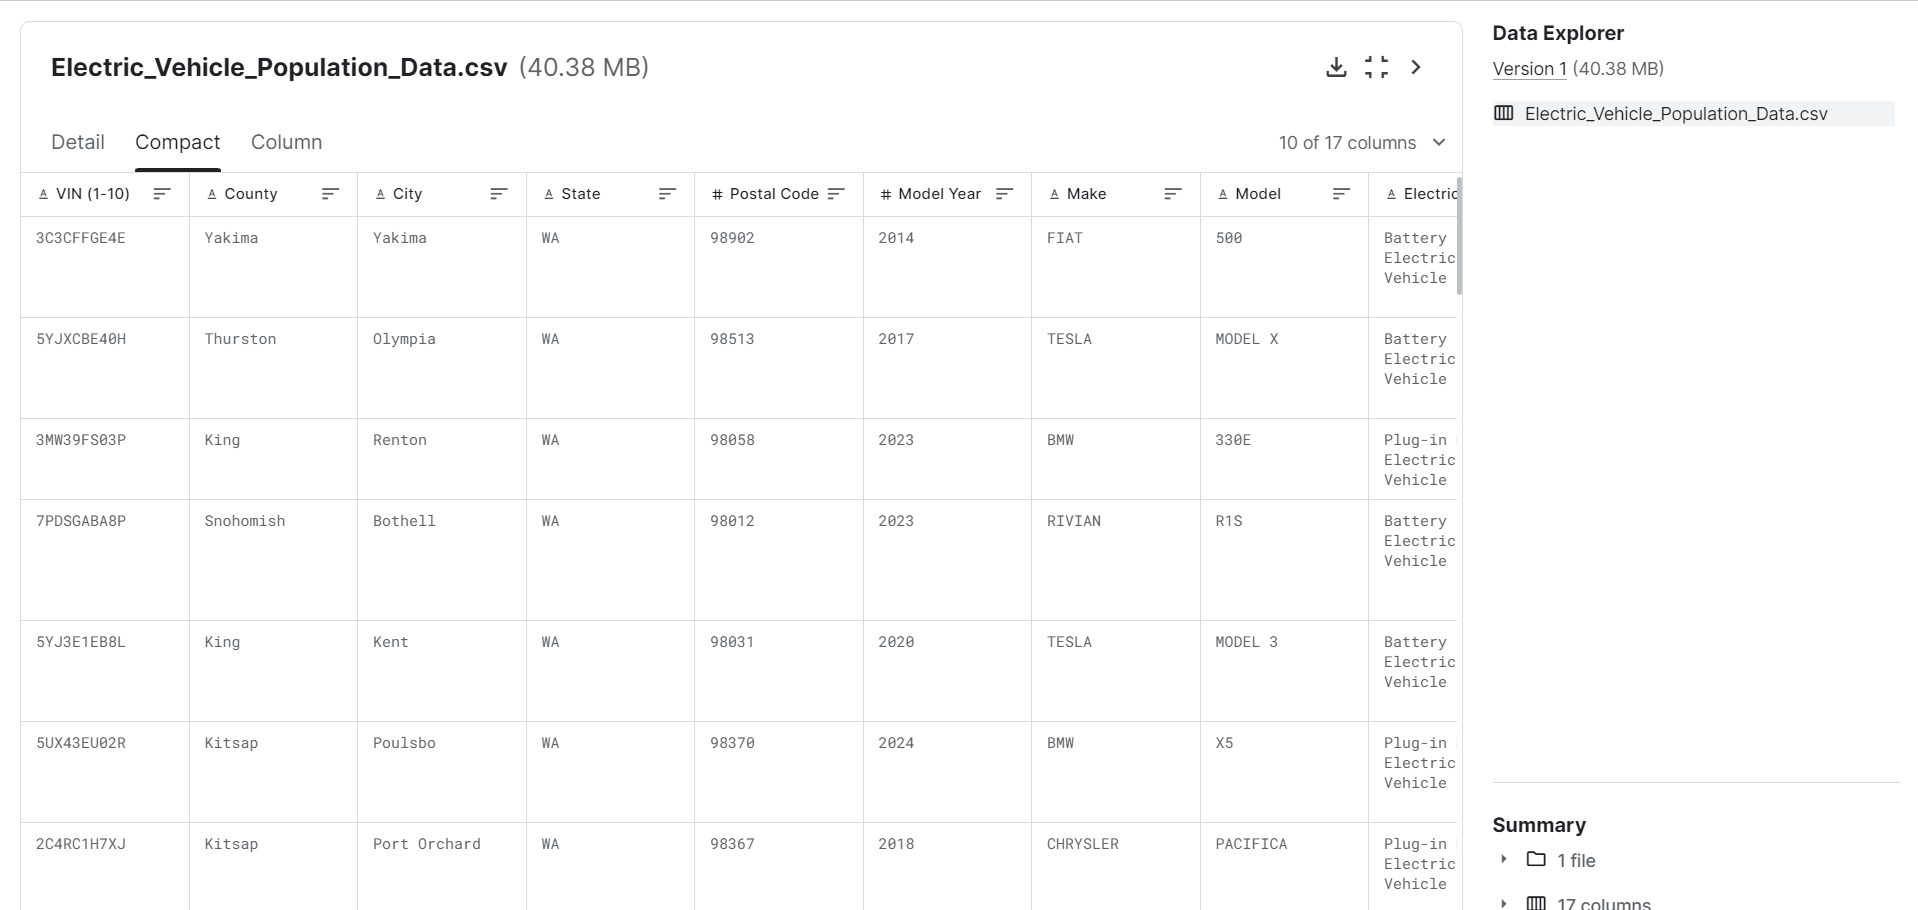
\includegraphics[width=\textwidth]{./imgs-latex/dataExplorer-csv-screenshot-img1.png}\label{fig:dataExplorer-csv-screenshot-img1}
\end{figure}
    

Luego se traduce los nombres de las columnas para tener una base de datos más organizada, debido a que nuestro proyecto Wattzfinder trabajará como un Sistema de recomendación basado en grafos se necesitará datos cuantitativos para poder utilizar diferentes métodos algorítmicos de grafos por datos cuantitativos, por ello se utilizará la biblioteca pandas para poder cargar la base de datos en un archivo csv en un DataFrame. 

Uno de los principales problemas de nuestra Dataset sacada de Kaggle es que en la columna de Precios la mayoría valores son = 0, lo cual no tendría sentido para nuestro sistema de recomendación de carros electrónicos, por lo que en el siguiente código se extraerán y reemplazarán los precios que son = 0 con los datos originales de Kaggle que != 0, se utilizarán los datos previos y se distribuirán en las filas necesarias de manera aleatoria, a su vez se utilizará percentiles para mantener la distribución general de precios de la dataset original y completar la mayoría de datos vacíos en la columna Precios.


Luego se generarán dos columnas adicionales por el mismo código: ``Descuentos'' y ``Precio Final''. Los descuentos se agregarán en un rango del 8\% al 40\%, y este descuento solo se aplicará a las filas con datos generados en la columna Precios. Es decir, los datos extraídos del dataset de Kaggle tendrán un descuento del 0\%. Este procedimiento se realiza con el propósito de que luego puedan ser identificables y permitir observar si existe alguna correlación imprevista cuando realicemos el análisis final de nuestro proyecto y, en su caso, corregir si existe algún error.


Aparte de utilizar la biblioteca \texttt{pandas} para los procesos relacionados con el archivo CSV, se utilizará \texttt{numpy} para el procesamiento de números en las 3 columnas modificadas en cuanto a la aleatoriedad y los percentiles.

En cuanto al código en general, se utilizarán las bibliotecas \texttt{sys} y \texttt{datetime} para traspasar el archivo con el script Python como argumento y modificar su nombre con la fecha respectiva del procesamiento de datos.

El código Python es el siguiente:

\begin{listing}[H]
\inputminted[
    frame=lines,
    framesep=2mm,
    baselinestretch=1.2,
    bgcolor=alice,
    fontsize=\footnotesize,
    linenos
]{python}{../scripts-to-process-data/add-2NewColumns-modify1Column.py}
\caption{Python script para agregar dos columnas nuevas y modificar una columna en una dataset.}
\label{lst:add-2NewColumns-modify1Column}
\end{listing}



\subsubsection{Características de los nodos}

El conjunto de datos utilizado proporciona información sobre una variedad de autos eléctricos y está compuesto por las siguientes características o atributos para cada elemento:

\begin{enumerate}
    \item \textbf{VIN:} Un número de identificación del vehículo (VIN) es el código de identificación de un automóvil específico.
    \item \textbf{País:} País dónde se fabrica.
    \item \textbf{Ciudad:} Ubicación de Empresa fabricante de Autos Eléctricos.
    \item \textbf{Código postal:} El código PIN es el sistema de numeración de la oficina postal utilizado por el servicio postal.
    \item \textbf{Año del modelo:} Año en el que se fabricó el automóvil.
    \item \textbf{Nombre de la empresa.}
    \item \textbf{Modelo:} El número de identificación del vehículo (VIN) es un código único de 17 dígitos específico para cada vehículo.
    \item \textbf{Tipo de vehículo eléctrico:} Generalmente nos referimos a tres tipos principales de vehículos eléctricos: vehículos eléctricos híbridos (HEV), vehículos eléctricos híbridos enchufables (PHEV) y vehículos eléctricos de batería (BEV).
    \item \textbf{Vehículo de combustible alternativo limpio:} Se pueden utilizar aceites vegetales, como palma, soja, girasol, maní y oliva, como combustibles alternativos para los motores diésel. Como combustible alternativo, el aceite vegetal es uno de los combustibles renovables.
    \item \textbf{Autonomía eléctrica:} Los vehículos totalmente eléctricos normalmente pueden recorrer entre 110 y más de 300 millas con una sola carga. Los PHEV normalmente pueden recorrer entre 15 y 60 millas solo con la energía de la batería; la capacidad del tanque de combustible determina su autonomía general porque el motor arranca cuando la batería se agota.
    \item \textbf{MSRP base:} Los fabricantes establecen un precio base para un automóvil o vehículo sin productos o características adicionales. El precio minorista sugerido por el fabricante (MSRP) es el precio base más funciones adicionales.
    \item \textbf{Distrito Legislativo:} La Legislatura de cada Estado puede estar compuesta por el Gobernador y la Legislatura Estatal. En algunos de los Estados la Legislatura estará compuesta por dos Cámaras, a saber, la Asamblea Legislativa y el Consejo Legislativo, mientras que en el resto habrá haya una sola Cámara, a saber, la asamblea legislativa.
    \item \textbf{ID de vehículo del DOL:} Un número de identificación único para cada vehículo está presente en el conjunto de datos de Transacciones. Las transacciones realizadas en el mismo vehículo tendrán la misma identificación de vehículo del DOL.
    \item \textbf{Ubicación del vehículo:} En los casos en que el vehículo fue diseñado para motores eléctricos, generalmente se ubican en la parte delantera y/o trasera entre las ruedas. Hay semiejes cortos que conectan la salida de los motores a las ruedas.
    \item \textbf{Servicio Eléctrico:} Una corporación, persona, agencia, autoridad u otra entidad o instrumento legal alineado con las instalaciones de distribución para el suministro de energía eléctrica para uso principalmente del público.
    \item \textbf{Área censal de 2020:} Las áreas censales son divisiones geográficas definidas para la tabulación de datos. Pueden ser divisiones geográficas de área pequeña relativamente permanentes de un condado o entidad estadísticamente equivalente definida para la tabulación y presentación de datos del censo decenal y otros programas estadísticos seleccionados.
    \item \textbf{Descuento:} Descuentos disponibles del vehículo.
    \item \textbf{Precio Final:} Precios final del vehículo eléctrico.
\end{enumerate}

\subsection{Propósito, limitaciones y alcances de los datos}

El propósito de recopilar y analizar este conjunto de datos es proporcionar recomendaciones personalizadas y relevantes de autos eléctricos a los usuarios a través de una plataforma web, con el fin de mejorar la satisfacción del cliente y aumentar las recomendaciones o ventas de la empresa. En este contexto, podemos explorar la siguiente pregunta: ¿Cómo podemos utilizar las relaciones entre los productos para ofrecer recomendaciones personalizadas a los usuarios?

\subsection{Identificación y representación de los nodos mediante grafos}

En nuestro proyecto, planeamos crear un grafo que consiste en 166 801 nodos, los cuales representarán las propiedades de cada elemento. Para representar esta estructura gráfica, los nodos se conectarán entre sí en función de su similitud en la categoría principal (auto eléctrico), utilizando el algoritmo que se enseñó en clase. Todo este proceso se llevará a cabo utilizando el lenguaje de programación Python.



\section{Propuesta}


\subsection{Objetivo General}

El objetivo de nuestro proyecto \textit{WatzzFinder} es desarrollar un sistema de recomendación avanzado basado en algoritmos de búsqueda en grafos. Este sistema representará y almacenará datos sobre vehículos eléctricos y sus interrelaciones de manera visual, permitiendo a los usuarios seleccionar el vehículo más adecuado según sus preferencias personales. Las características clave de los nodos que se utilizarán incluyen:
\begin{itemize}
    \item Año del modelo,
    \item Nombre de la empresa,
    \item Modelo,
    \item MSRP base,
    \item Servicio Eléctrico,
    \item Descuento,
    \item Precio Final.
\end{itemize}



\subsection{Objetivos Específicos}

\begin{itemize}
    \item Implementar técnicas de recorrido en grafos, como BFS (Búsqueda por Amplitud) y DFS (Búsqueda por Profundidad), para explorar las conexiones entre diferentes nodos representando vehículos y características de usuario.
    \item Utilizar variantes de DFS, como DLS (Búsqueda por Profundidad Limitada) y IDS (Búsqueda por Profundidad Iterativa), para optimizar la exploración de grafos bajo diferentes condiciones de búsqueda.
    \item Implementar algoritmos de grafos optimizados para manejar y procesar eficientemente un el volumen de datos de usuarios y vehículos eléctricos.
    \item Modelar relaciones complejas y múltiples entre entidades, no solo de manera directa entre los usuarios ante los objetos de compras sino también capturar interacciones e influencias indirectas.
    \item Proveer una interfaz de usuario que sea fácil de usar y que ayude a visualizar y entender cómo se generan las recomendaciones.
\end{itemize}

\section{Procesamiento y Metodologías}

\subsection{Justificación de la Metodología}


Para este proyecto se estará utilizando técnicas de recorrido y búsqueda en grafos como la principal metodología debido a su eficiencia en manejar relaciones complejas. Se emplearán métodos específicos que incluyen:

\begin{itemize}
    \item \textbf{Búsqueda por Profundidad Limitada (DLS)} y \textbf{Búsqueda por Profundidad Iterativa (IDS)}: Estos métodos se aplicarán para explorar eficazmente el espacio de nodos del grafo, permitiendo identificar conexiones profundas entre características de vehículos. Dado que se procesará una gran cantidad de nodos (más de 160,000), estos métodos heurísticos son útiles para controlar la profundidad de búsqueda en grafos potencialmente grandes, asegurando que el sistema sea tanto eficiente como capaz de encontrar soluciones óptimas bajo restricciones específicas.
    \item \textbf{Algoritmo de Dijkstra modificado (A-Star)}: Se utilizará para encontrar el camino más corto o de menor costo entre dos nodos, lo que permite calcular las recomendaciones más relevantes basadas en múltiples factores ponderados. Este enfoque es dependiente de las diferentes características del carro electrónico. A su vez, se ha observado que en algunas modificaciones del algoritmo se ha utilizado para sistemas de recomendación de películas (Lubos, Fritscher, \& Kriz, 2013) de la siguiente manera:
    
    \begin{figure}[htbp]
        \centering
        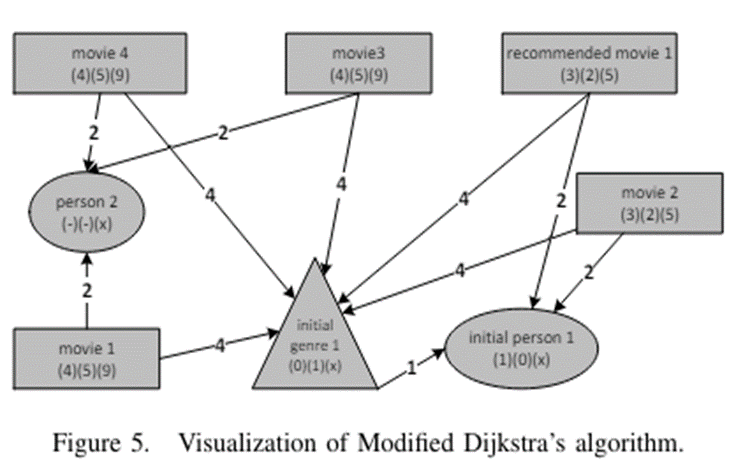
\includegraphics[width=\textwidth]{./imgs-latex/ejemplo-casos1-DijkstraModificado.png}
        \caption{Ejemplo de aplicación del algoritmo de Dijkstra modificado.}
        \label{fig:ejemplo-casos1-DijkstraModificado}
    \end{figure}
    
\end{itemize}



\subsubsection*{Aplicaciones de Algoritmos Avanzados}
\begin{itemize}
    \item \textbf{Algoritmo de Agrupamiento Espectral}: Basado en la descomposición espectral del Laplaciano del grafo (Javi, 2020), es excelente para capturar la estructura de datos de alta dimensión. Se utilizará para segmentar el mercado de usuarios, resultando en una segmentación final del mercado que depende de las dinámicas entre el usuario y el producto.
    \item \textbf{Algoritmo de Comunidad de Louvain}: Será efectivo para detectar comunidades dentro de grafos grandes y podría ser utilizado para identificar grupos de usuarios con preferencias similares y realizar recomendaciones grupales (Carazo \& Amat, 2023). Este enfoque dependerá de la compra anterior de cada usuario.
\end{itemize}

La utilización de estos diferentes algoritmos en nuestro proyecto dependerá del objetivo específico, ya sea en recomendaciones basadas en múltiples factores específicos ponderados del mercado, segmentación de mercados o las previas compras de los usuarios.



\subsection{Preparación y modelado de Datos}
\begin{enumerate}
    \item[a.] Adquirir los datos necesarios de la dataset de Kaggle \textit{Electric Vehicle Population Dataset} con sus respectivas 16 características. 
    \item[b.] Escribir un programa en Python para generar datos faltantes de la columna MSRP base, aumentar 2 columnas adicionales de Descuento y Precio Final en el archivo \.csv de la dataset.
    \item[c.] Construir el grafo donde cada nodo representa un vehículo eléctrico y las aristas reflejan las relaciones basadas en las 18 características / variables finales. Los usuarios también se modelarán como nodos.
\end{enumerate}


\subsection{Algoritmos de Grafos de búsqueda}
\begin{itemize}
    \item Implementación de UCS y A-Star para calcular las rutas más eficientes en costos y características, facilitando recomendaciones personalizadas.
    \item Aplicación de DLS y IDS para una exploración efectiva del grafo, identificando posibles recomendaciones basadas en la profundidad de búsqueda iterativa y limitada.
\end{itemize}


\subsection{Implementación de código en Python}
Se hará el uso de las siguientes librerías:
\begin{itemize}
    \item \textbf{NetworkX:} Se utilizará NetworkX, para la creación, manipulación y estudio de la estructura, dinámicas y funciones de grafos complejos. Esta herramienta es ideal para manejar nuestro grafo de 166 801 nodos. También será utilizado para calcular métricas de grafos, como la centralidad y la detección de comunidades.
    \item \textbf{Numpy:} Se utilizará Numpy para la generación de datos faltantes en las columnas que originalmente vienen en la dataset de Kaggle y para la generación de datos para las nuevas columnas.
    \item \textbf{Matplotlib:} Se utilizará para crear gráficos estadísticos informativos para poder realizar retroalimentaciones basadas en Métricas de Evaluación. Además de realizar los grafos necesarios que complementen NetworkX.
    \item \textbf{Pandas:} Se utilizará para la manipulación y gestión del conjunto de datos. Esta biblioteca facilitará la adición de nuevas columnas como 'Descuentos' y 'Precio Final', permitiendo la manipulación precisa de datos tabulares. Además, será utilizada para aplicar transformaciones específicas como el llenado de datos faltantes y la implementación de operaciones condicionales basadas en los valores existentes. Se prevé que se continuará utilizando dicha biblioteca para la manipulación general de los datos, análisis y modelado posterior de la dataset.
\end{itemize}

\section{Métricas de Evaluación}
\begin{enumerate}
    \item Porcentaje de Usuarios que realizan compras basadas en Recomendaciones Personalizadas.
    \item Tiempo Promedio empleado en Búsqueda y recomendaciones calculando el tiempo medio que los usuario pasan desde que ingresan al sistema hasta que encuentren el vehículo finalmente comprado.
\end{enumerate}
\subsection{Big O - evaluacion con tiempos}
tomar capturas de pantalla y calcular con diferentes soluciones y cantidad de nodos.

\subsection{Mejora continua y Evaluación de Feedback}
\begin{itemize}
    \item Ajuste de Algoritmos: Los algoritmos y heurísticas serán ajustados y afinados regularmente basándose en los resultados obtenidos de las métricas de evaluación. Sirve para mejorar continuamente la precisión y la eficiencia del sistema de recomendaciones.
    \item Feedback de Usuarios: Se establecerán canales de comunicación con los usuarios para recoger sus opiniones y sugerencias de manera sistemática.
\end{itemize}




\section{Diseño del aplicativo}
\subsection{Diagrama de clase y diagrama de base de datos}

Diagrama de Clases
\begin{figure}[htbp]
    \centering
    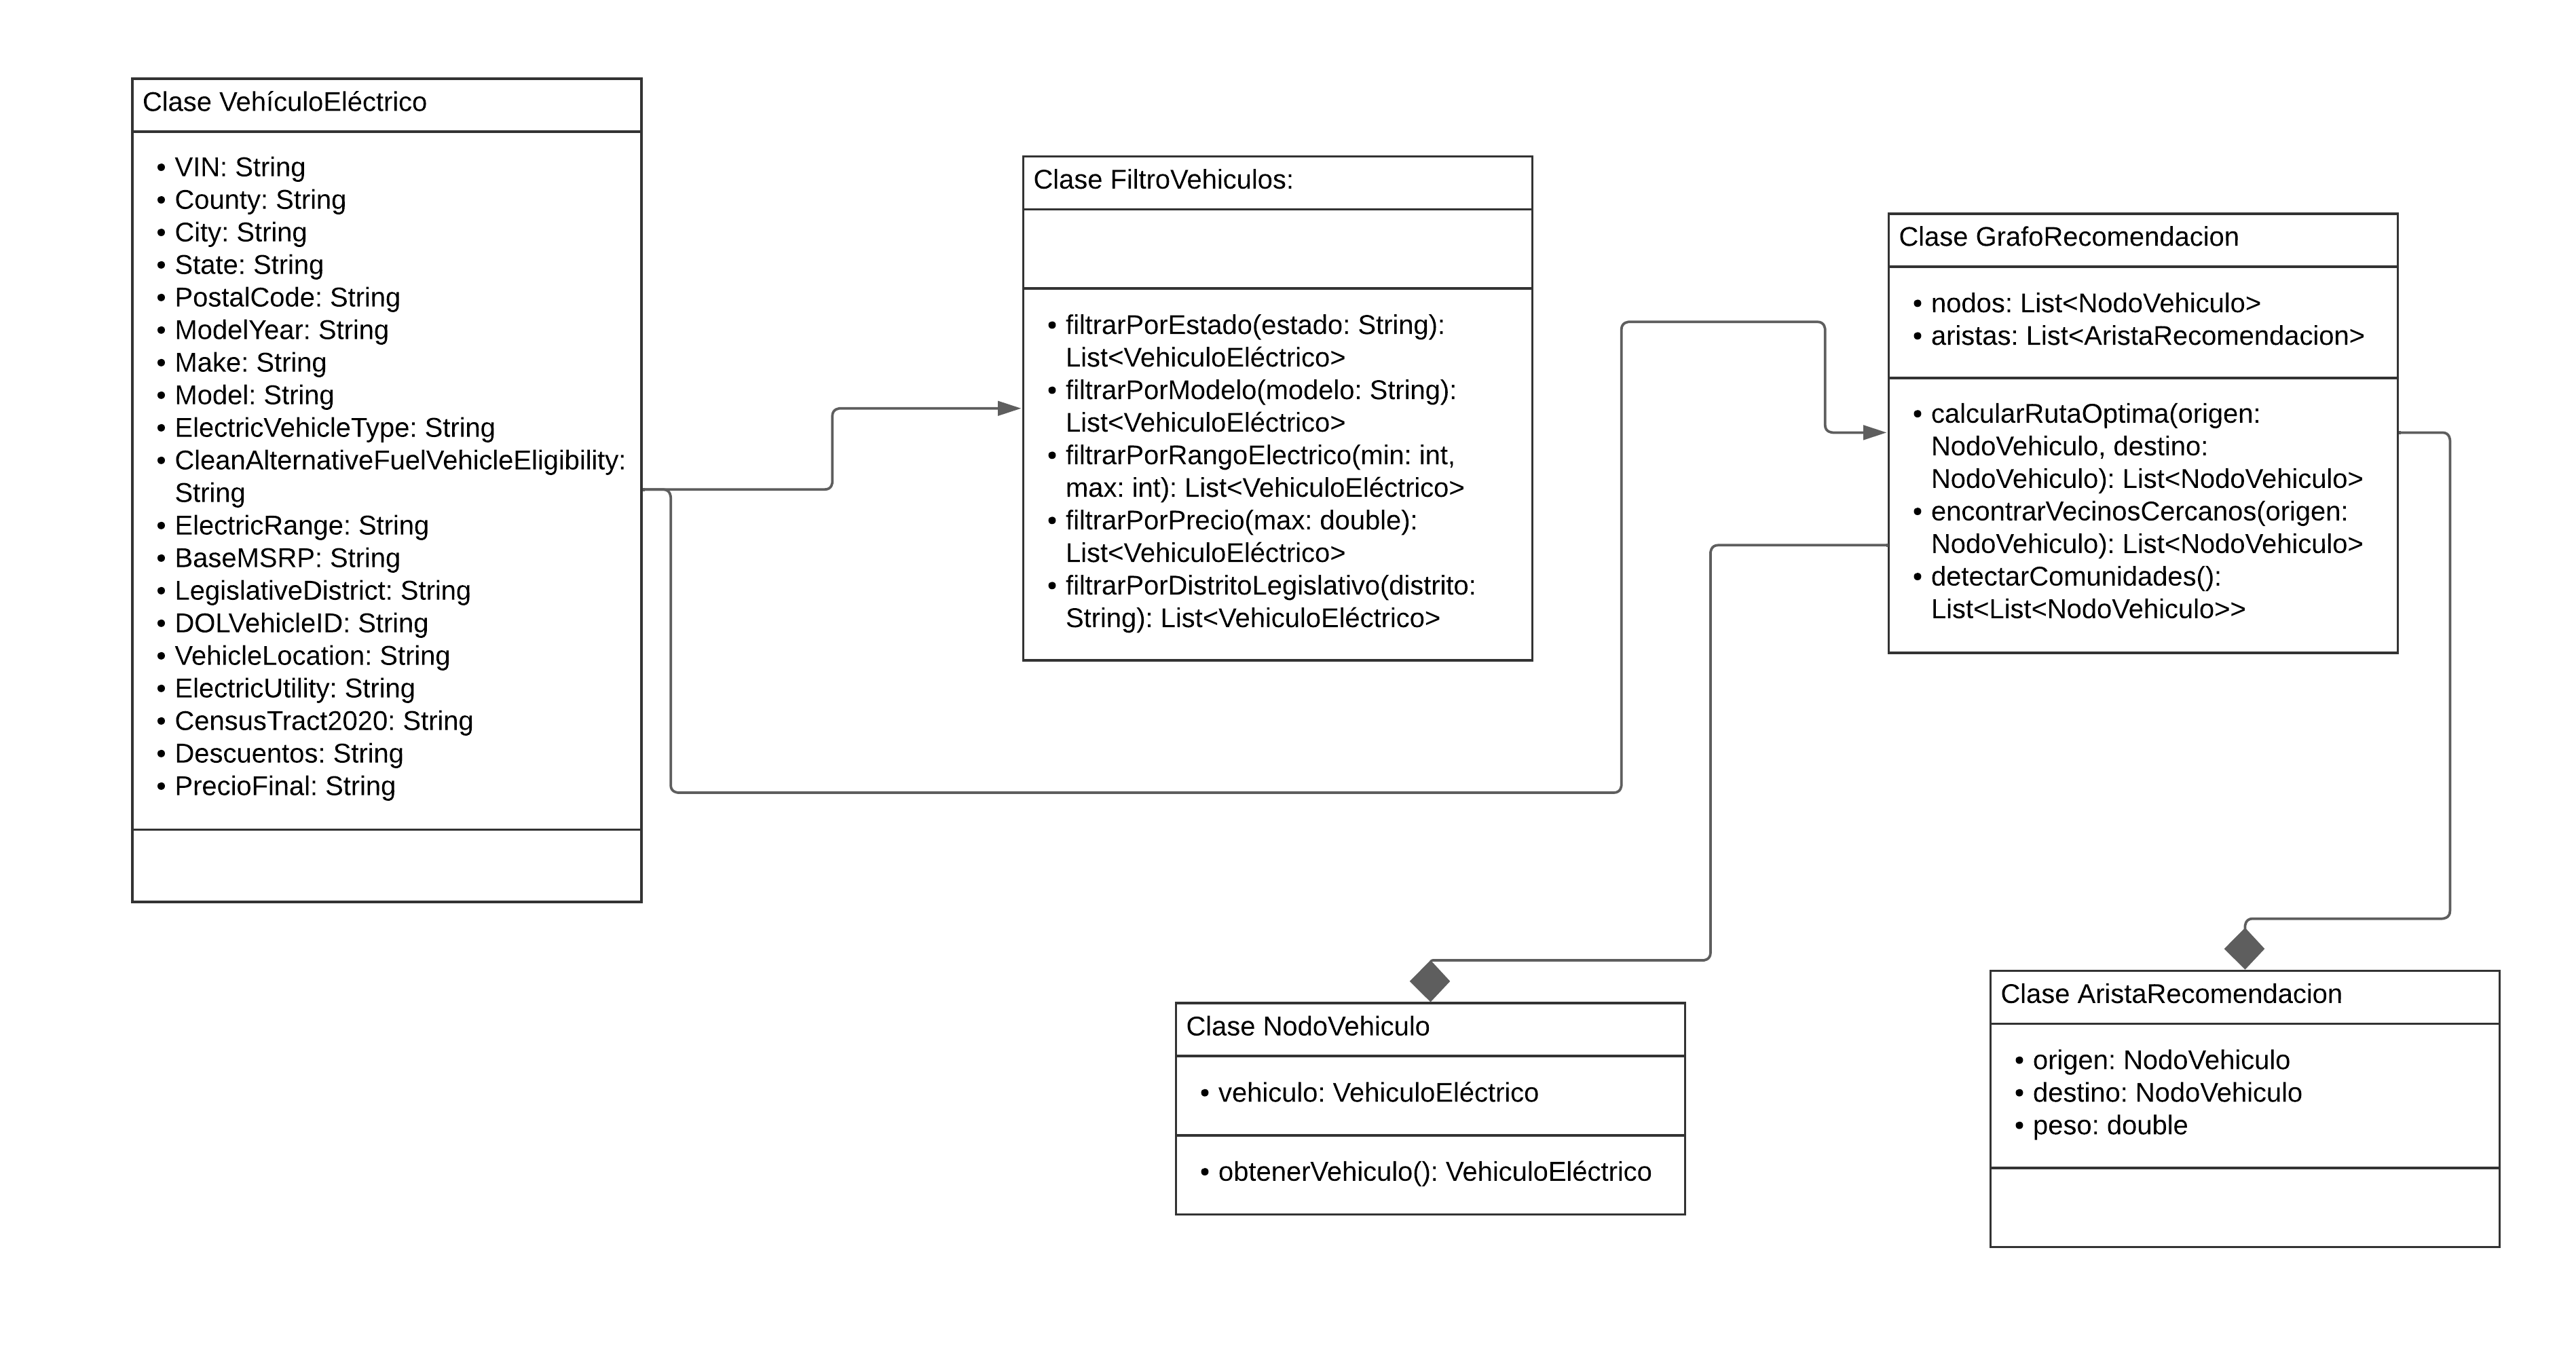
\includegraphics[width=\textwidth]{./imgs-latex/diagramadeclases.png}\label{fig:diagramadeclases}
\end{figure}

Diagrama de Base de Datos
\begin{figure}[htbp]
    \centering
    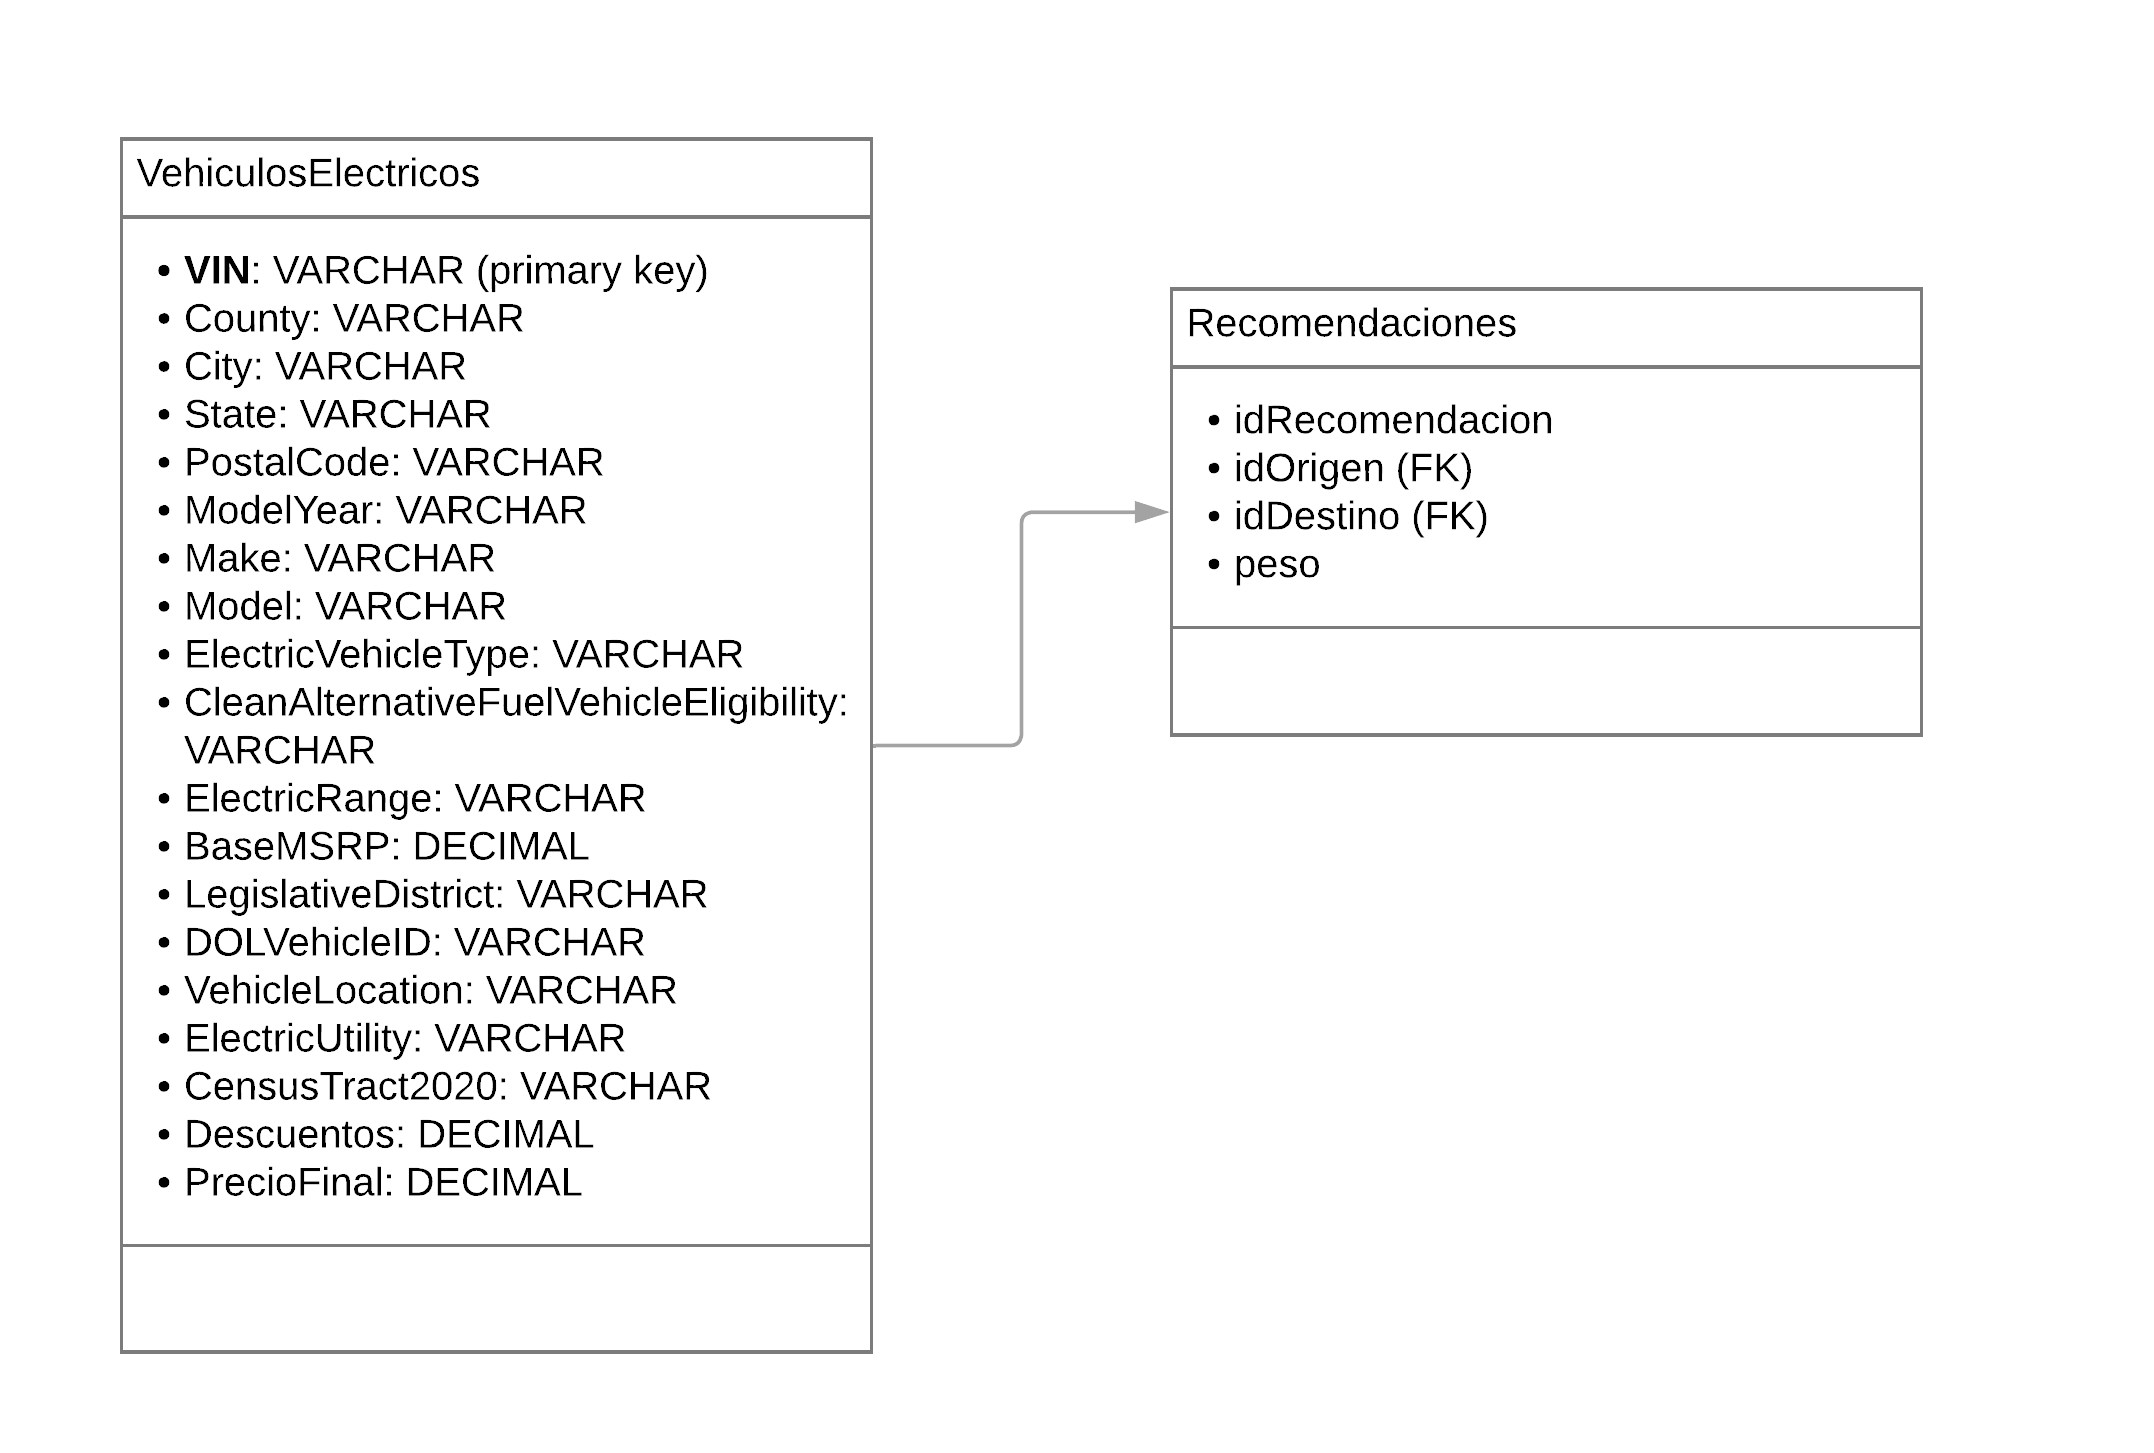
\includegraphics[width=\textwidth]{./imgs-latex/diagramadebase.png}\label{fig:diagramadebase}
\end{figure}


\subsection{Módulo para la adecuación de datos fuente a estructura de datos tipo grafo}
\subsection{Módulo para la representación de datos en el grafo}
\subsection{Interfaz tentativa (visual) para usuarios}

Pantalla Principal
\begin{figure}[htbp]
    \centering
    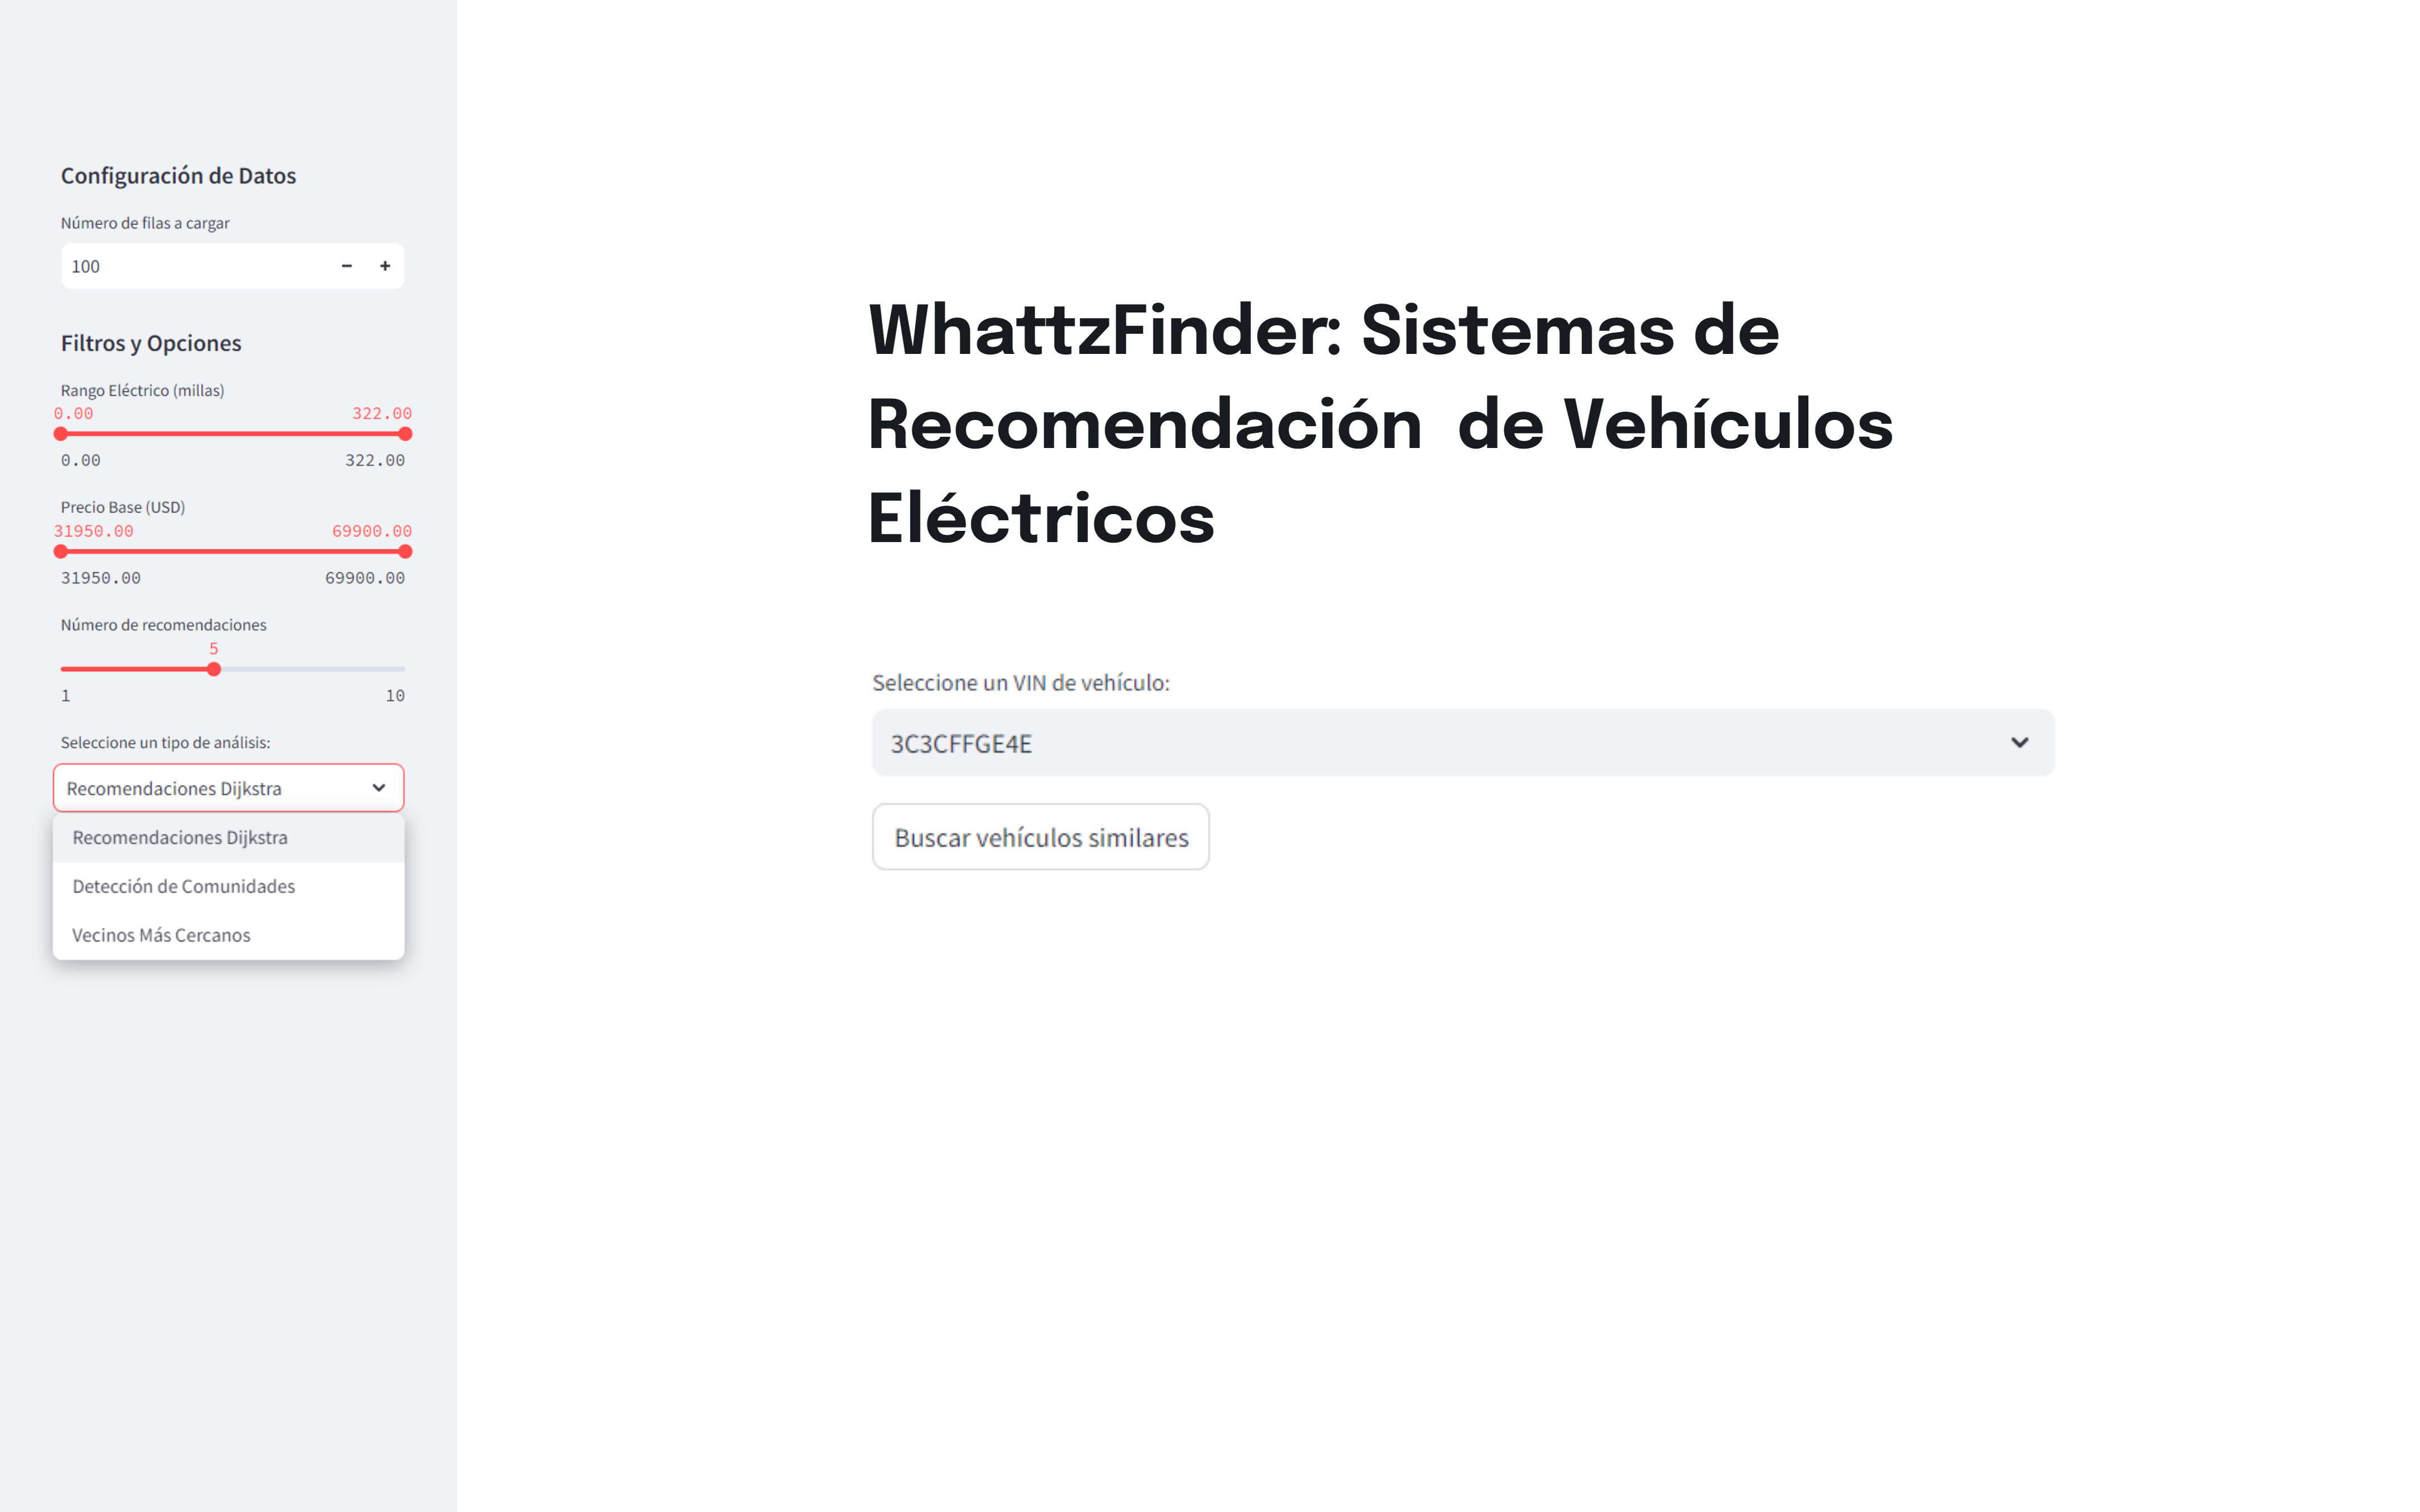
\includegraphics[width=\textwidth]{./imgs-latex/img1.png}\label{fig:img1}
\end{figure}

Opciones de Análisis
\begin{figure}[htbp]
    \centering
    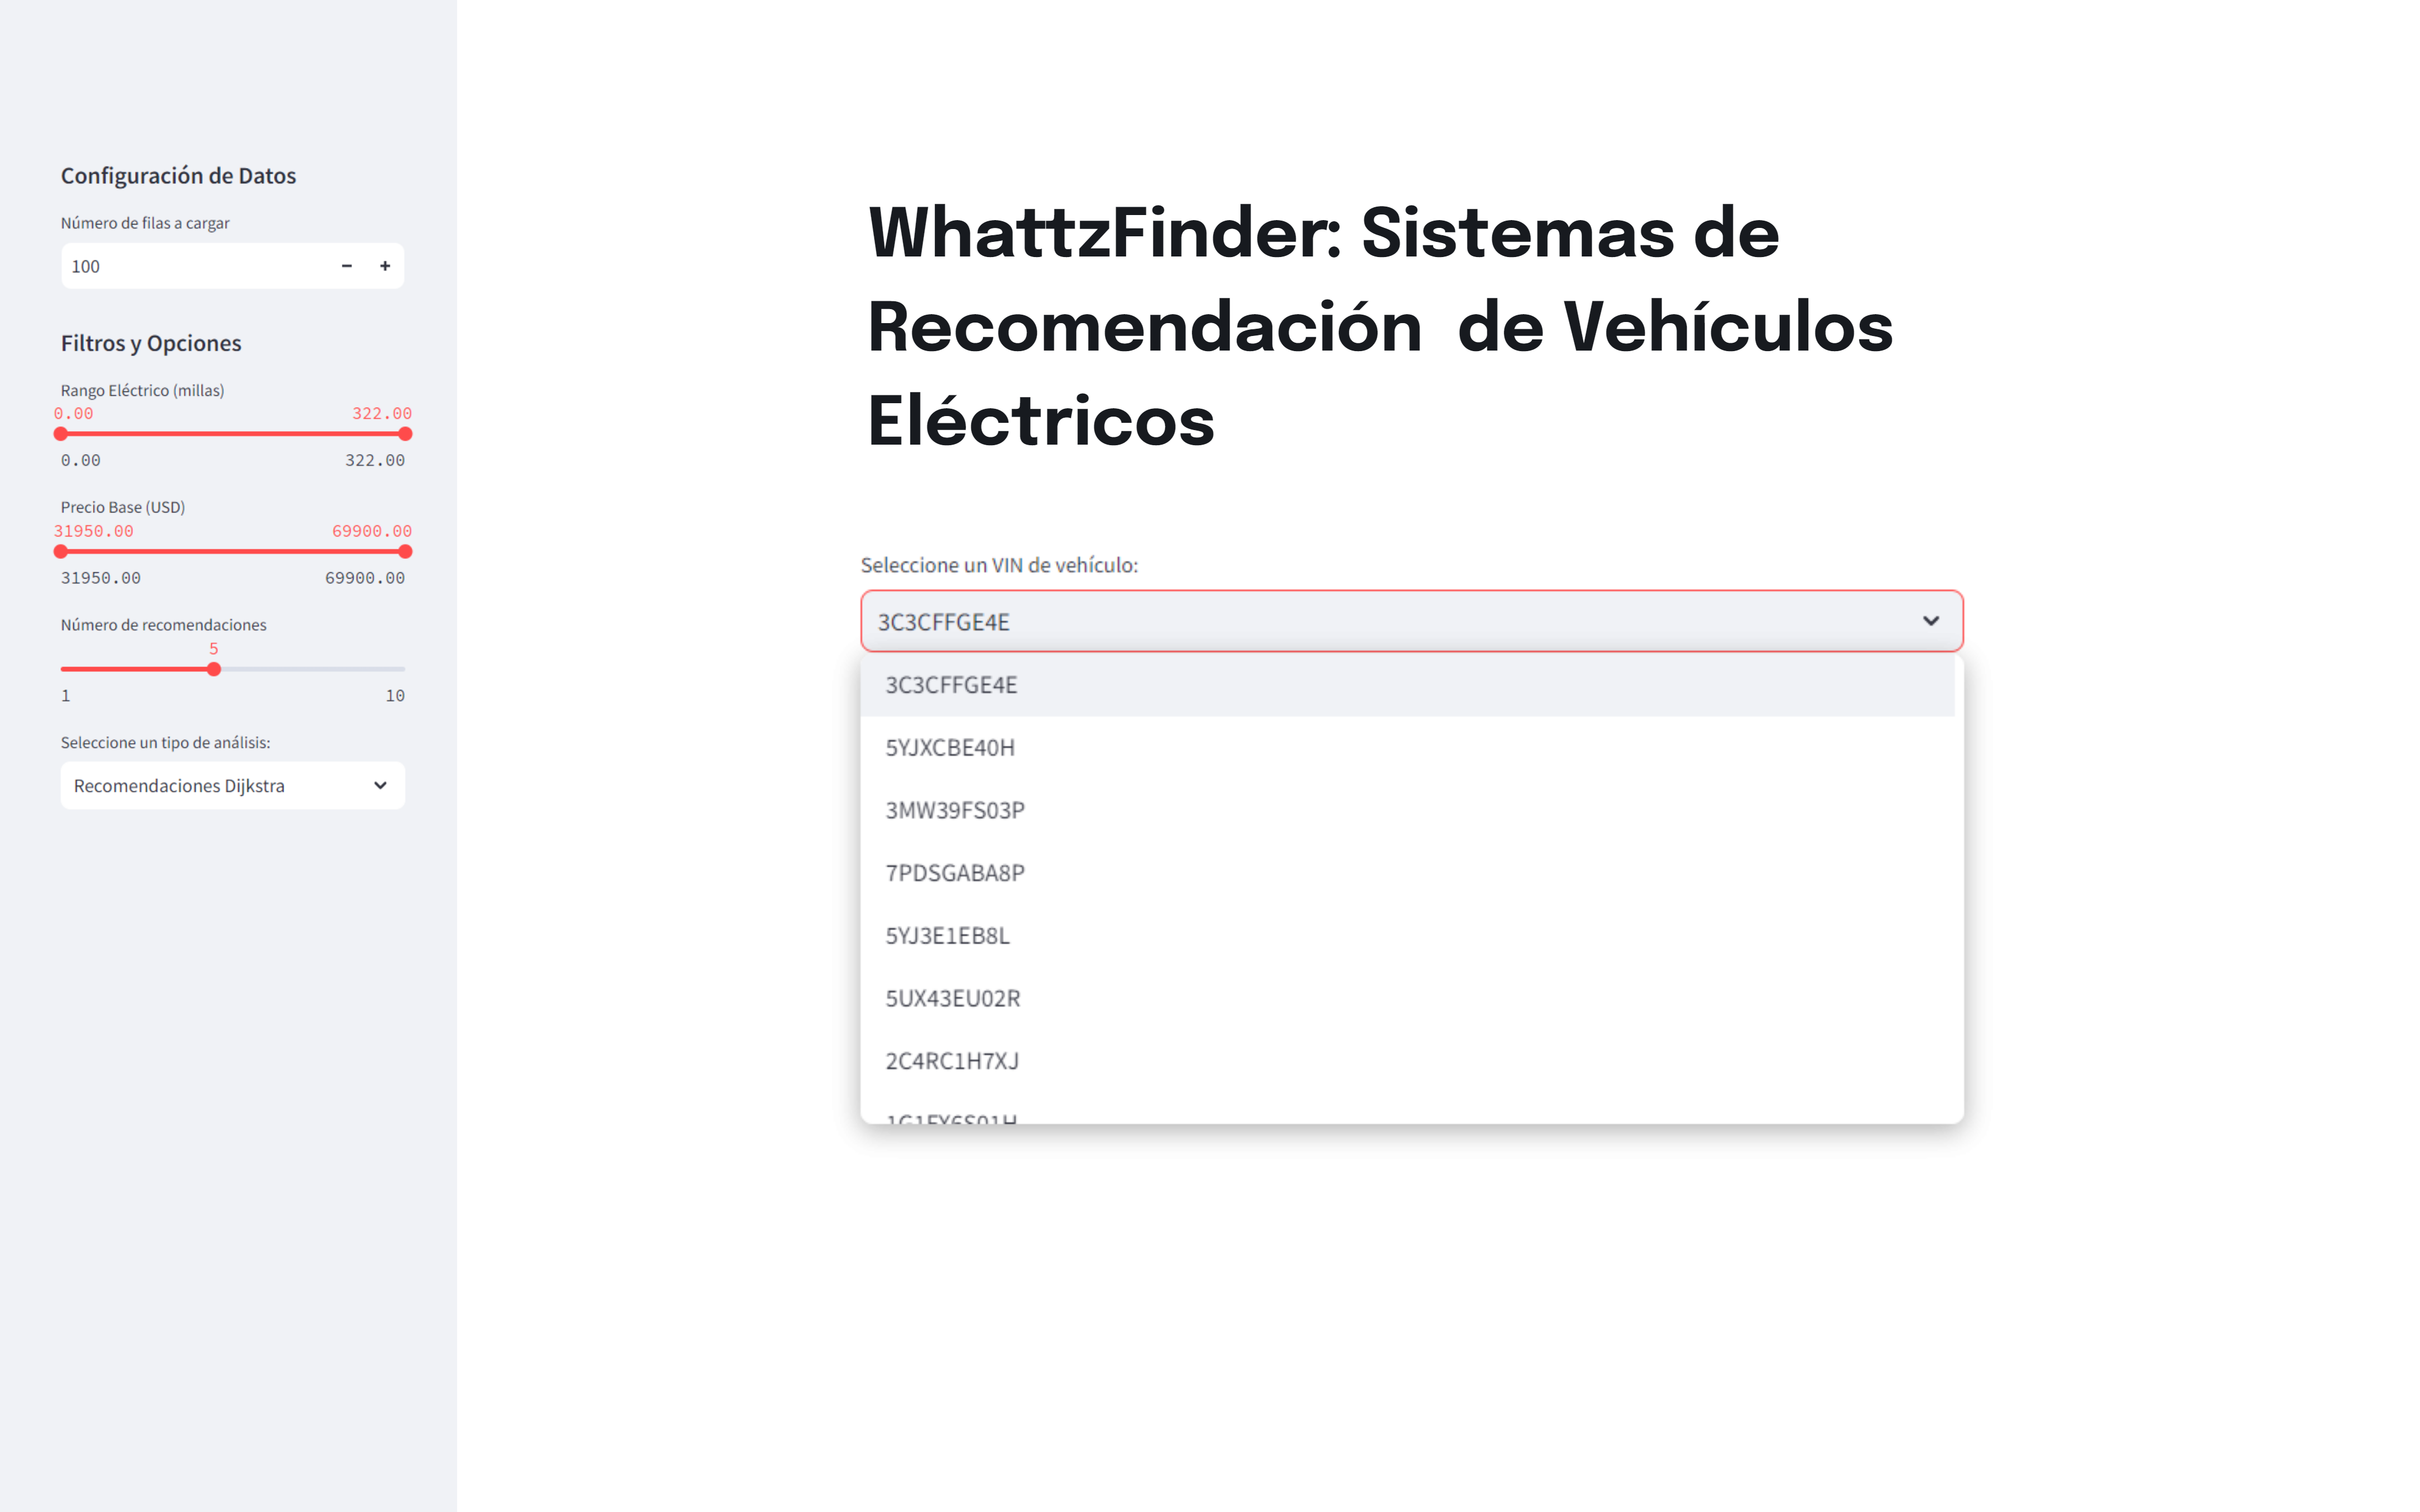
\includegraphics[width=\textwidth]{./imgs-latex/img2.png}\label{fig:img2}
\end{figure}

Selecion de Vehículo por ID
\begin{figure}[htbp]
    \centering
    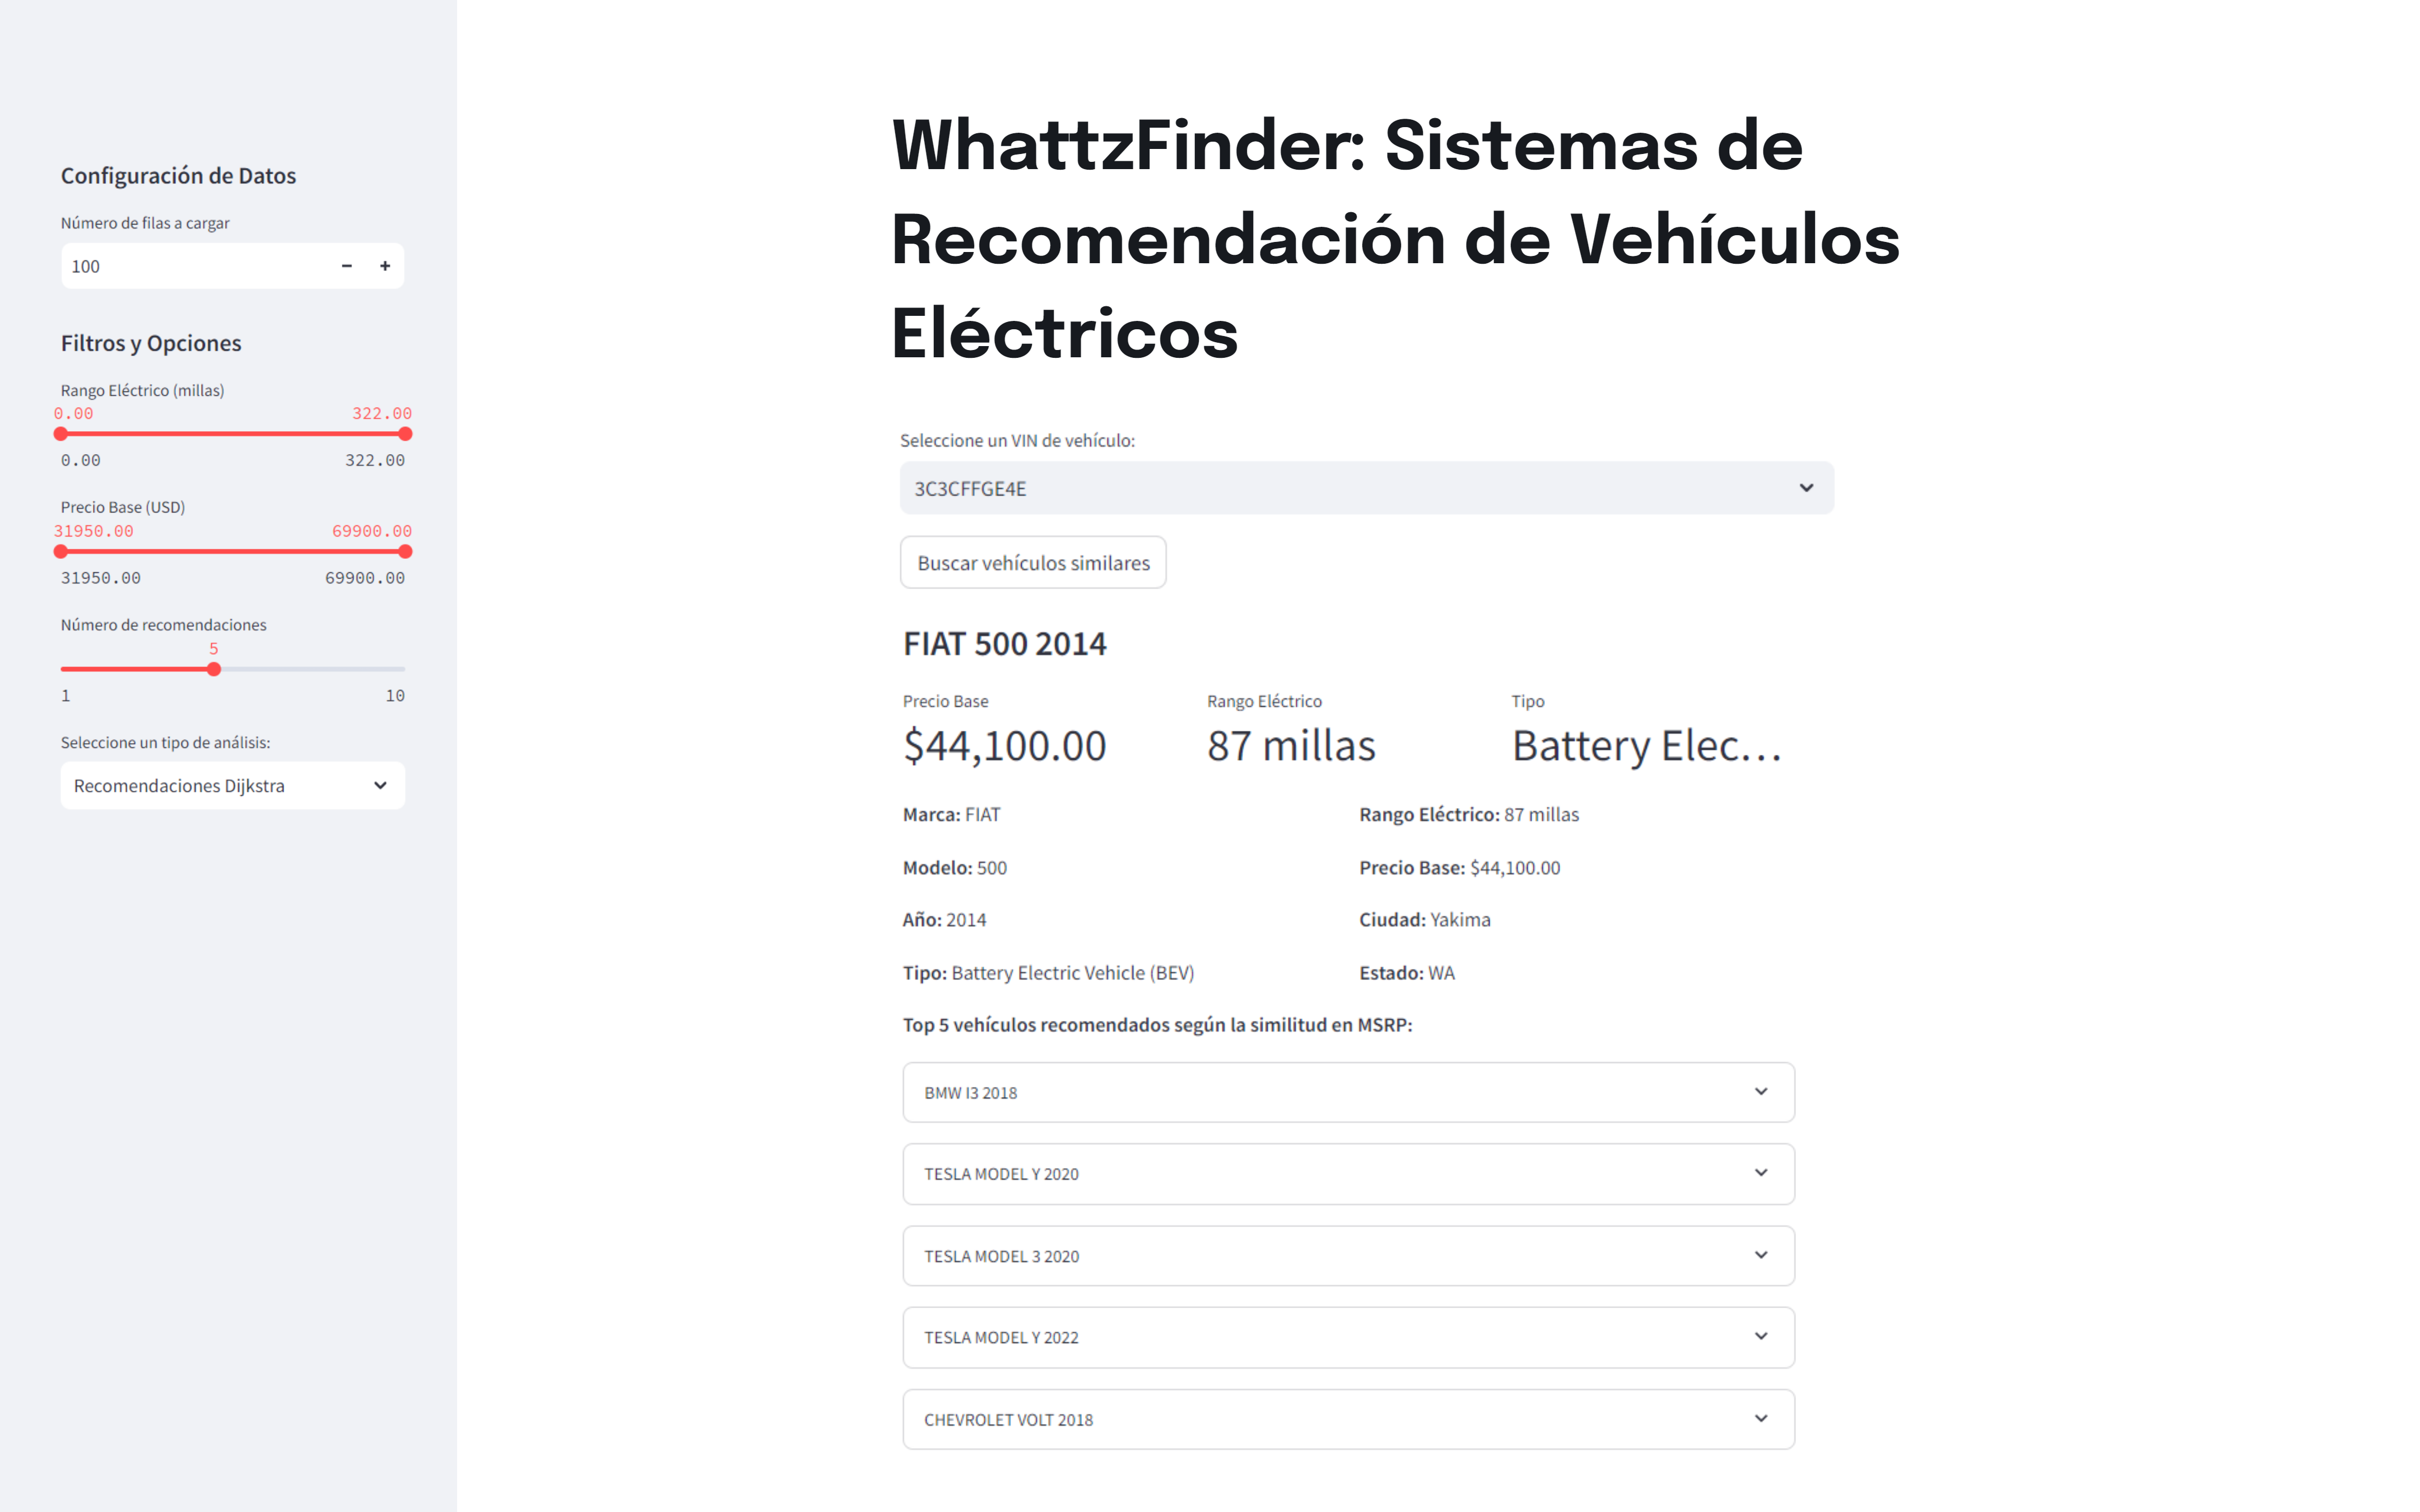
\includegraphics[width=\textwidth]{./imgs-latex/img3.png}\label{fig:img3}
\end{figure}

Resultados de Búsqueda - Datos
\begin{figure}[htbp]
    \centering
    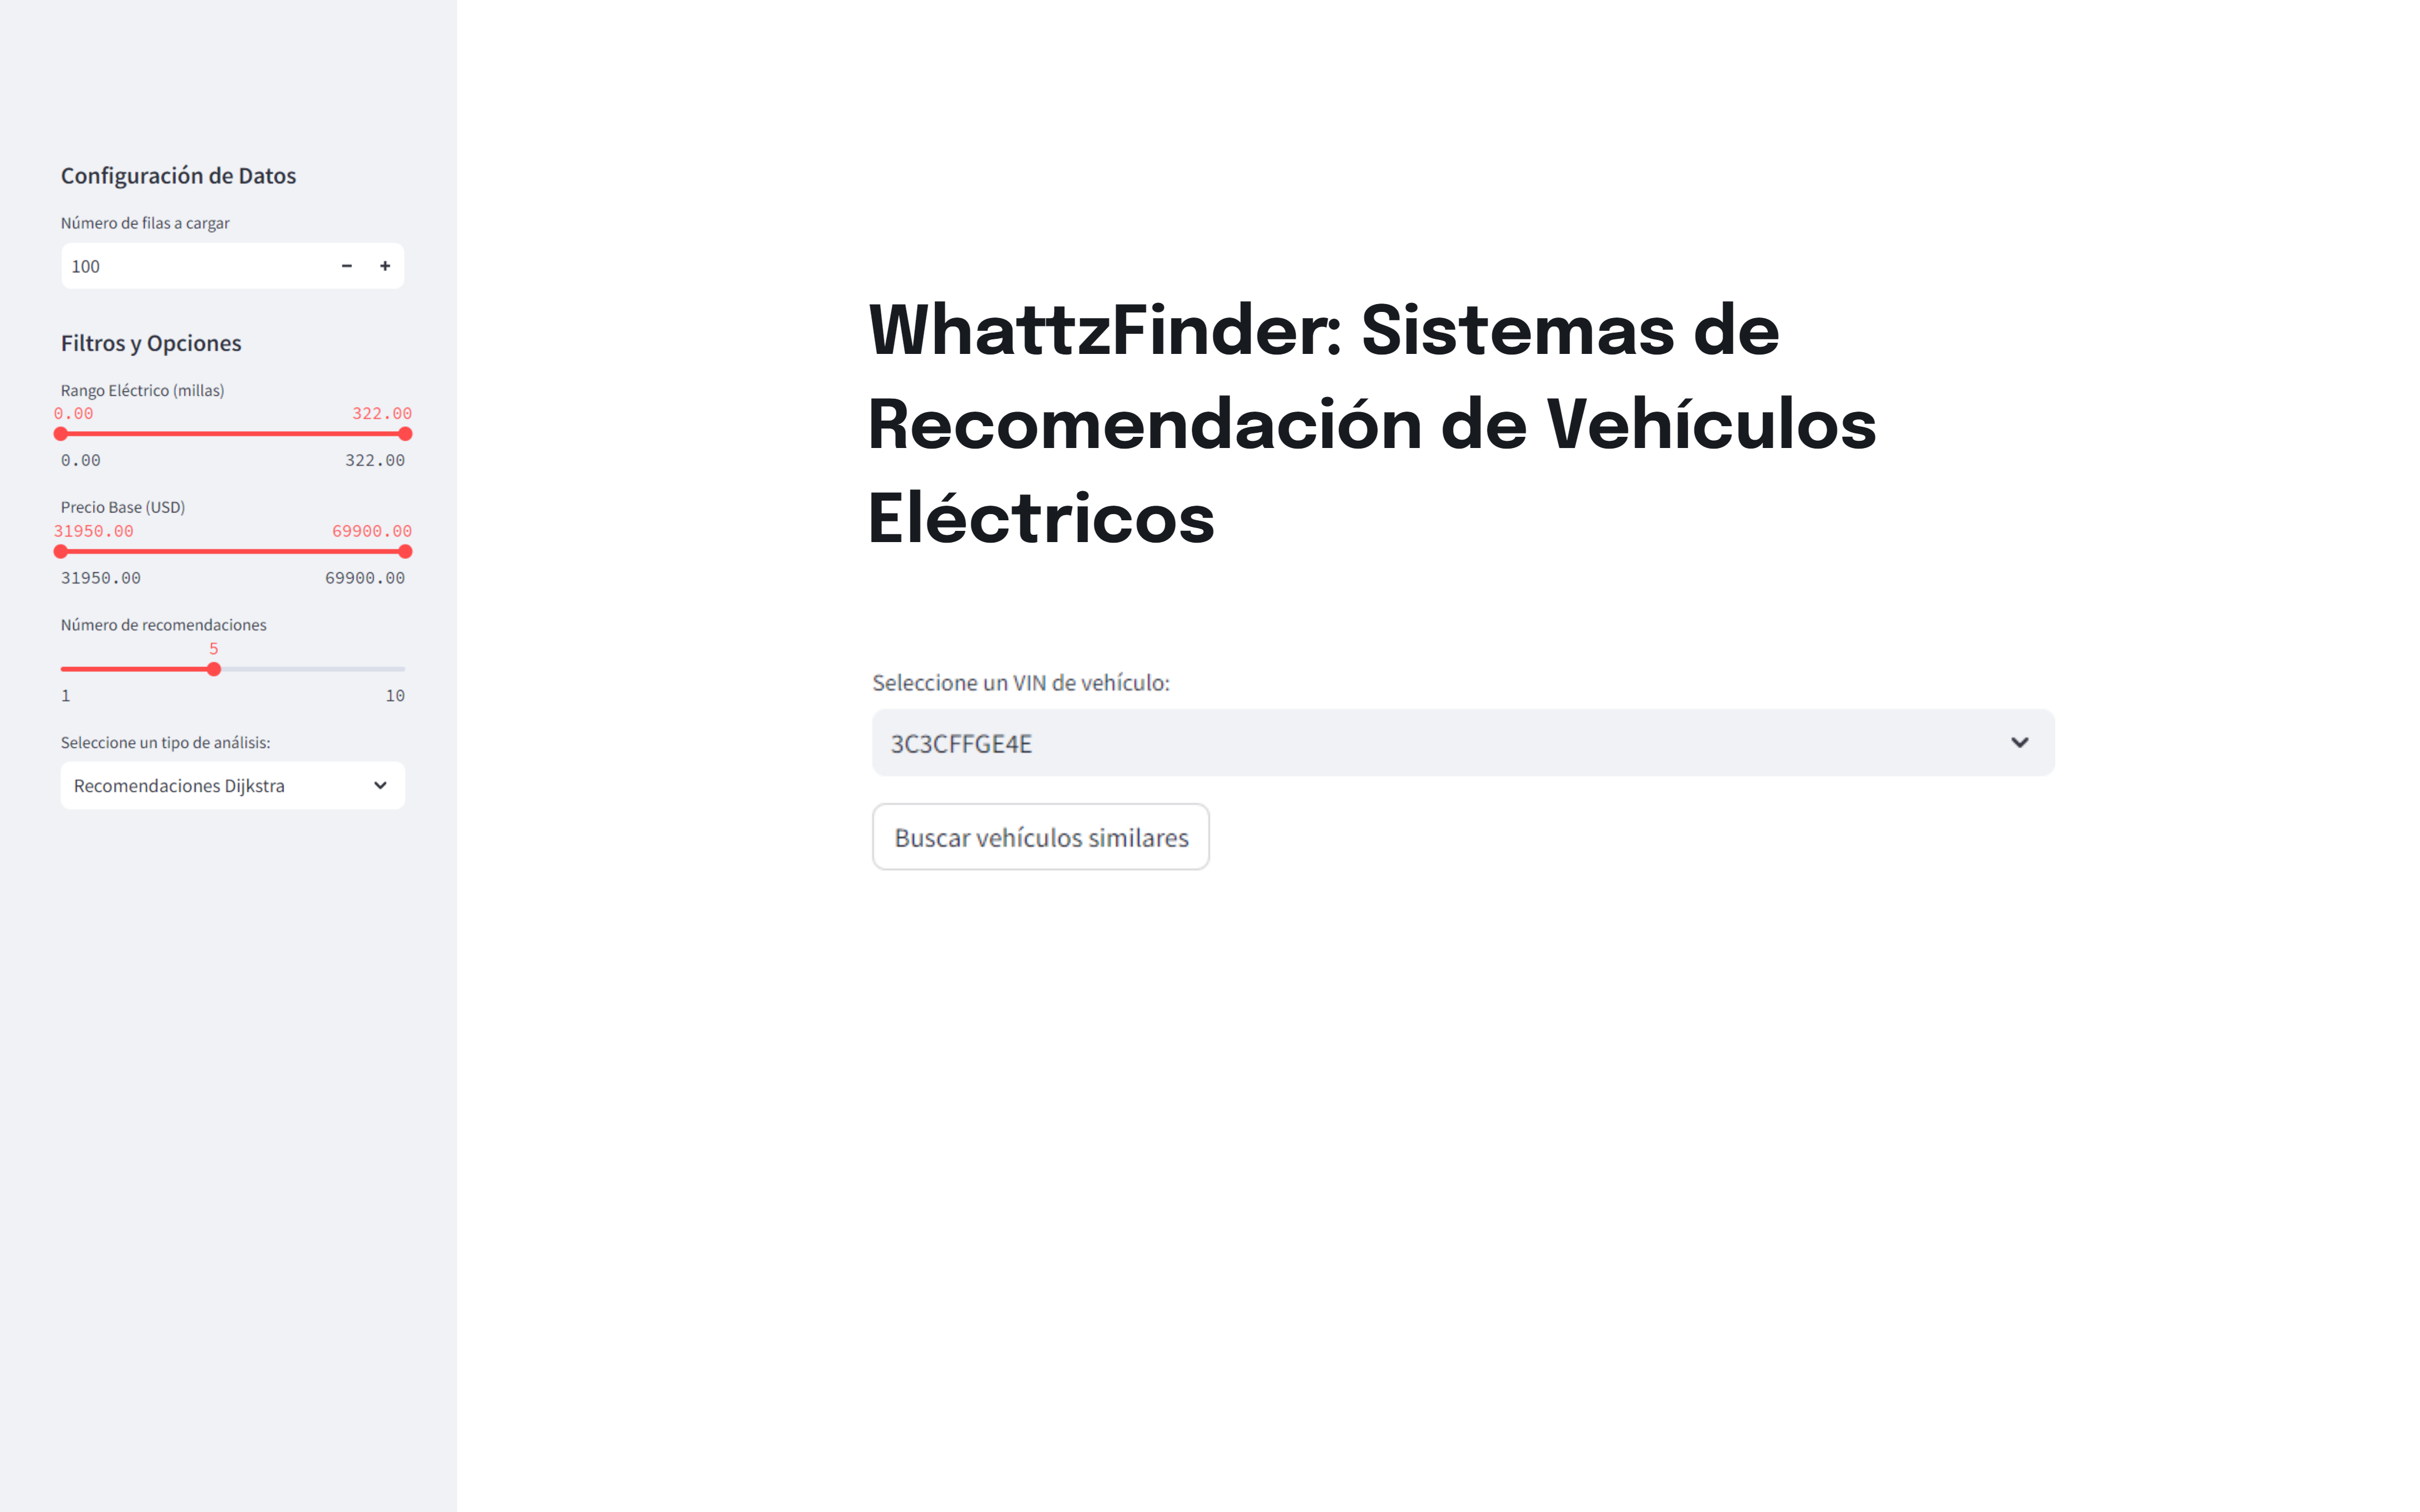
\includegraphics[width=\textwidth]{./imgs-latex/img4.png}\label{fig:img4}
\end{figure}

Resultados de Búsqueda - Vehículos
\begin{figure}[htbp]
    \centering
    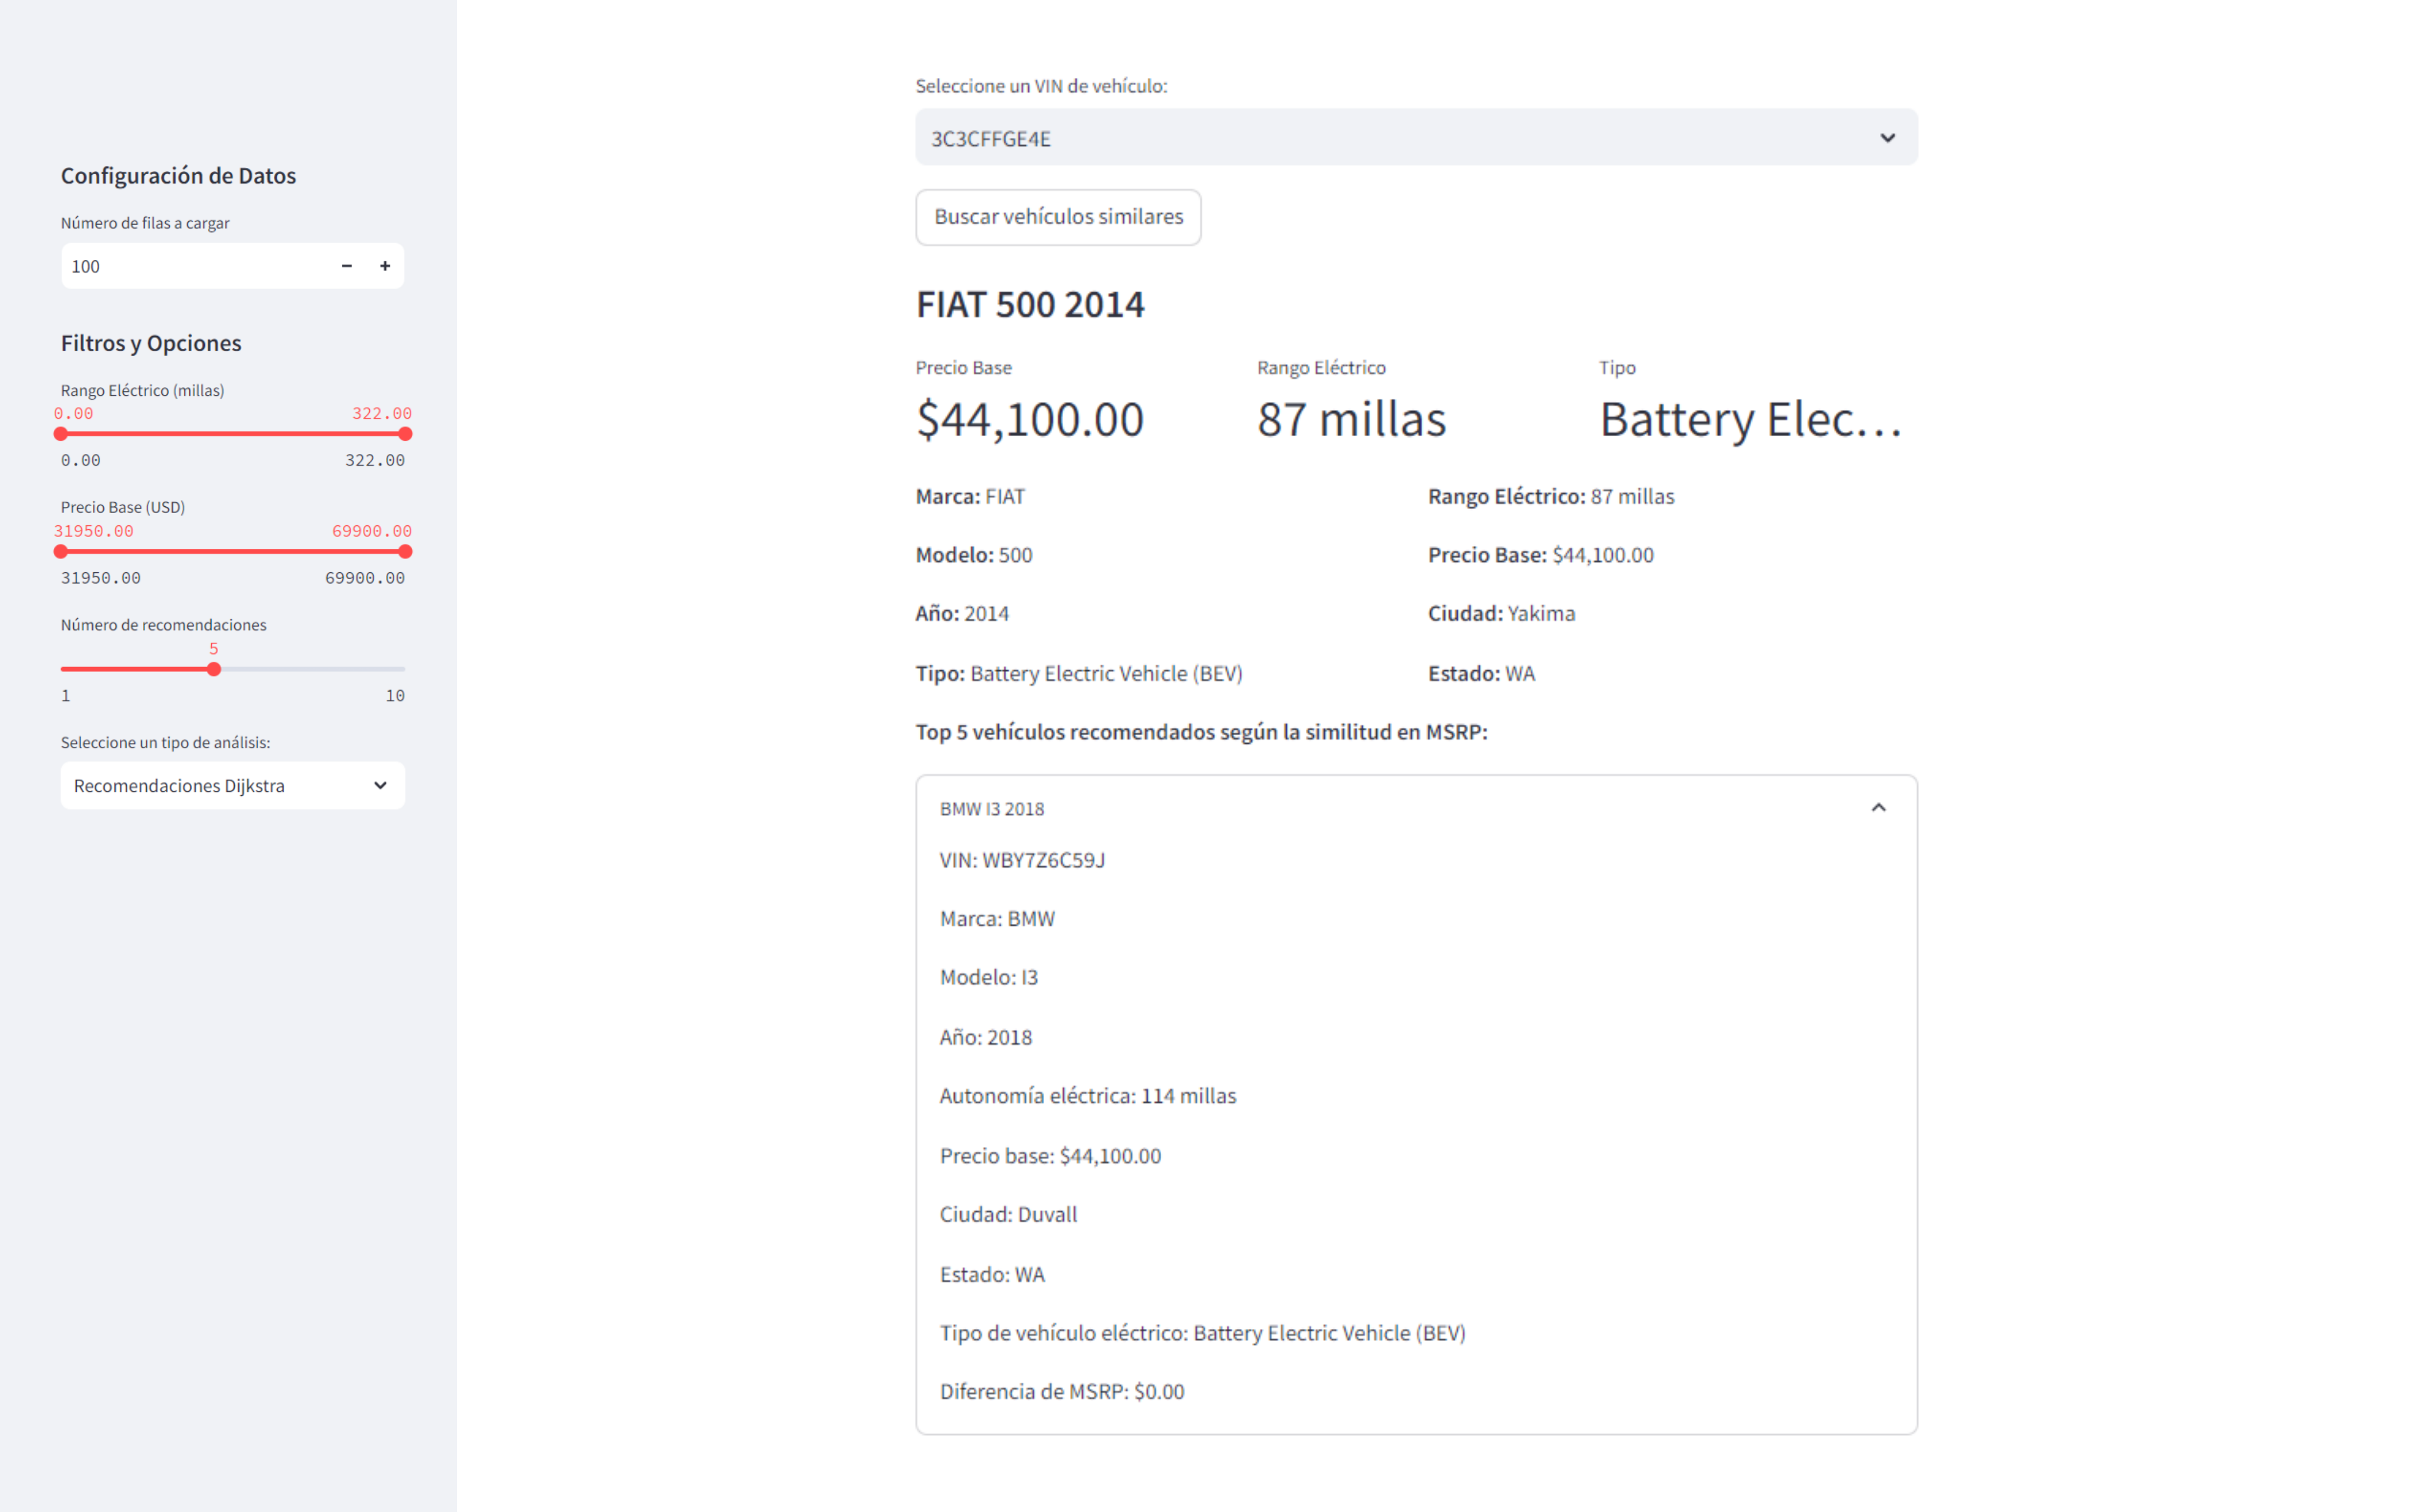
\includegraphics[width=\textwidth]{./imgs-latex/img5.png}\label{fig:img5}
\end{figure}

Resultados de Búsqueda - Gráfo
\begin{figure}[htbp]
    \centering
    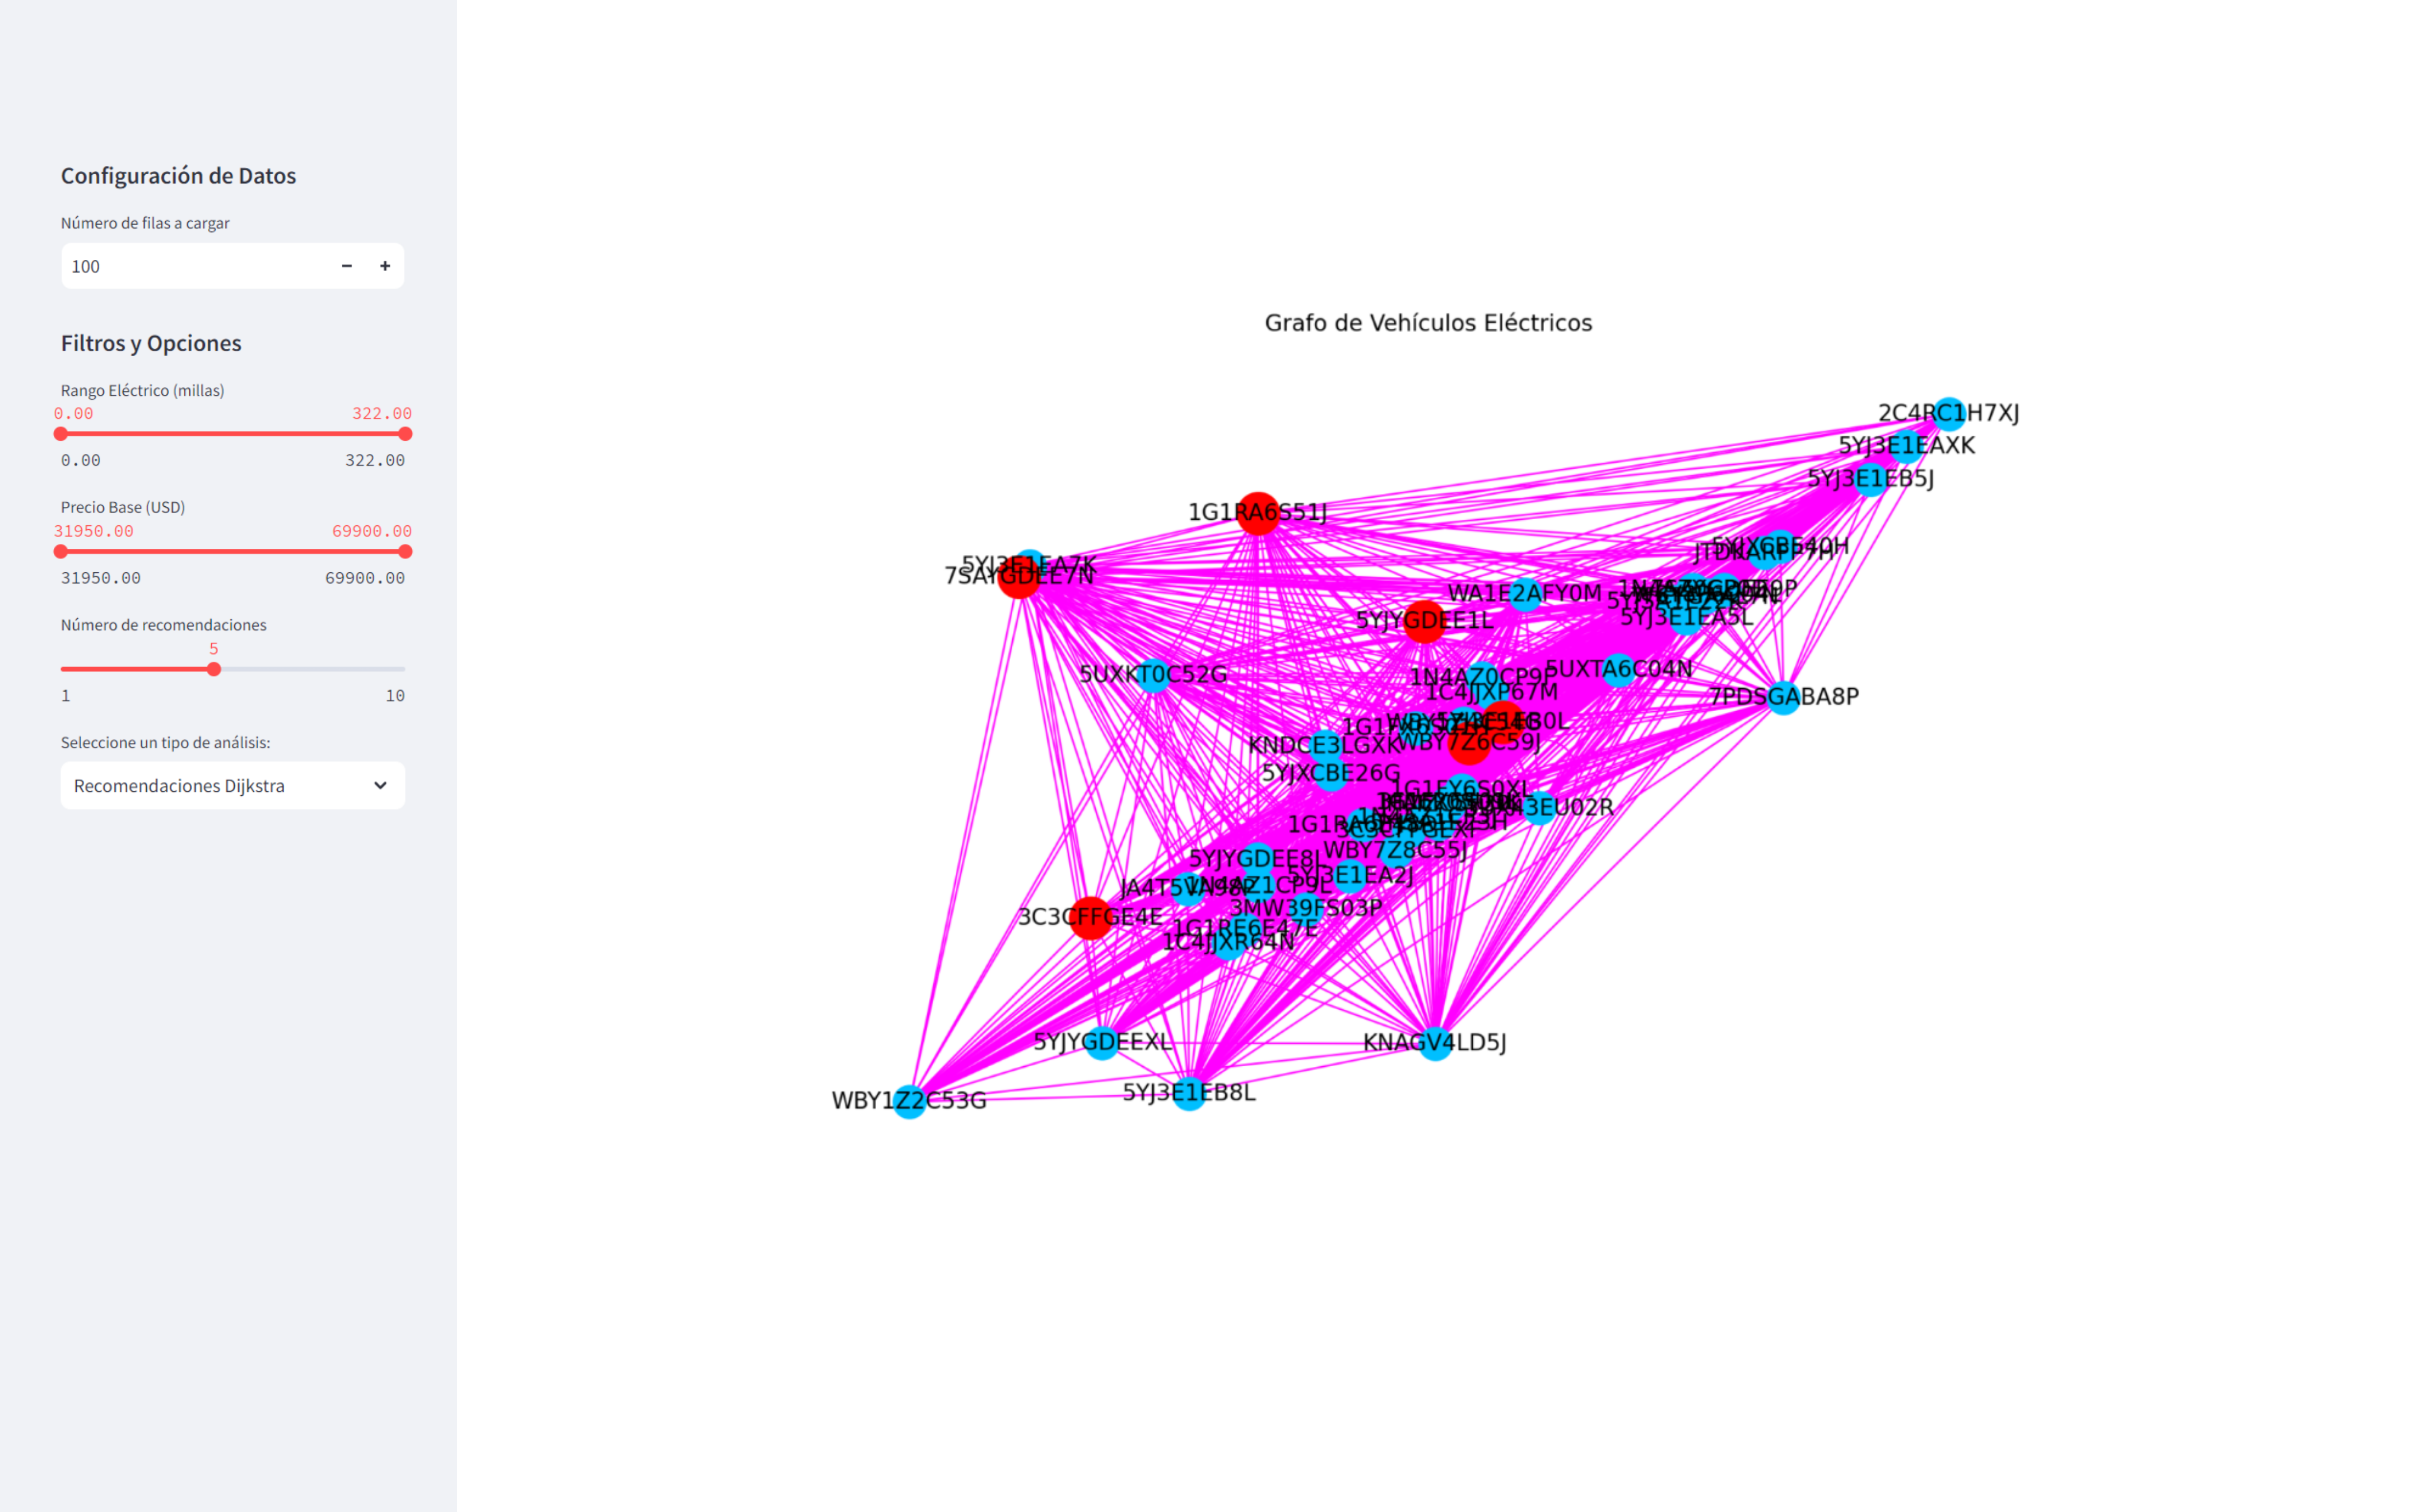
\includegraphics[width=\textwidth]{./imgs-latex/img6.png}\label{fig:img6}
\end{figure}

Link de Prototipo:

\url{https://app.visily.ai/projects/2326925d-fd9e-4656-ab45-2f8d65f10693/boards/569223}


\section{Validación de resultados y pruebas}
Validamos los resultados a través de\...

\section{Conclusiones}
La recomendación de vehículos es crucial en las ventas online, ya que ayuda a los usuarios a encontrar el auto adecuado según sus necesidades individuales. El uso de un sistema en grafos permite modelar las relaciones entre diferentes autos de manera eficiente, representando las similitudes entre ellos y permitiendo una comparación fácil para que los usuarios elijan según su presupuesto y necesidad.

\begin{itemize}
    \item La recomendación de vehículos es crucial en las ventas online, ya que ayuda a los usuarios a encontrar el auto adecuado según sus necesidades individuales.
    \item El uso de un sistema en grafos permite modelar las relaciones entre diferentes autos de manera eficiente, representando las similitudes entre ellos y permitiendo una comparación fácil para que los usuarios elijan según su presupuesto y necesidad.
    \item El sistema puede utilizar algoritmos de búsqueda en el grafo para encontrar todos los autos disponibles que cumplan con las especificaciones del usuario, como marca, año, y modelo.
    \item Los automóviles son esenciales como medio de transporte personal, especialmente en áreas con transporte público limitado o poco eficiente.
\end{itemize}



\section{Referencias bibliográficas}
\begin{itemize}
    \item Pigna, A. (2023, 26 septiembre). \textit{¿Para qué sirve el auto? Utilidad, función y ventajas}. Kavak. Available at: \url{https://www.kavak.com/mx/blog/para-que-sirve-el-auto-utilidad-funcion-y-ventajas}
    \item Carazo, F., \& Amat, J. (2023, Abril). \textit{Detección de comunidades en grafos y redes con python}. Available at: \url{https://cienciadedatos.net/documentos/pygml02-detecion-comunidades-grafos-redes-python}
    \item Javi, G. (2020, Agosto 28). \textit{Spectral Clustering}. Available at: \url{https://javi897.github.io/Spectral_clustering/}
    \item Lubos, D., Fritscher, E., \& Kriz, J. (2013). \textit{Movie Recommendation Based on Graph Traversal Algorithms}. Available at: \url{http://www2.fiit.stuba.sk/~bielik/publ/abstracts/2013/televido-dexa2013.pdf}
\end{itemize}

\end{document}